%% Generic single-column journal submission template (article class)
%% Compatible with Elsevier / Springer / Wiley / arXiv / IEEE Access
%% Wide-Scale Sampling with Hard-Argmin Selection and CBF Projection
\documentclass[11pt,onecolumn,a4paper]{article}

\usepackage[margin=1in]{geometry}
\usepackage{amsmath,amssymb,amsfonts,amsthm}
\usepackage{graphicx}
\usepackage{booktabs}
\usepackage{multirow}
\usepackage{array}
\usepackage[noend]{algpseudocode}
\usepackage{algorithm}
\usepackage{cite}
\usepackage{url}
\usepackage{authblk}
\usepackage{lineno}
\usepackage{caption}
\usepackage{titlesec}
\usepackage{xcolor}
\usepackage[toc,page]{appendix}
\usepackage{hyperref}
\hypersetup{colorlinks=true,linkcolor=black,citecolor=black,urlcolor=black}

% Line numbers for peer review
\linenumbers
\renewcommand{\linenumberfont}{\normalfont\scriptsize\sffamily\color{gray}}

% Section heading style (numbered Section 1, 1.1, 1.1.1)
\titleformat{\section}{\normalfont\Large\bfseries}{\thesection.}{0.6em}{}
\titleformat{\subsection}{\normalfont\large\bfseries}{\thesubsection}{0.6em}{}
\titleformat{\subsubsection}{\normalfont\normalsize\bfseries}{\thesubsubsection}{0.6em}{}

% Caption style
\captionsetup{labelfont=bf,font=small,labelsep=period}

% Allow wider line breaking tolerance to suppress Overfull \hbox on
% paragraphs with long \texttt{} identifiers and URLs
\sloppy
\tolerance=2000
\emergencystretch=10pt

\newtheorem{proposition}{Proposition}
\newtheorem{remark}{Remark}

% Shorthand
\newcommand{\R}{\mathbb{R}}
\newcommand{\E}{\mathbb{E}}
\newcommand{\Nm}{N_{\mathrm{MC}}}
\newcommand{\spt}{\mathrm{sp}}
\newcommand{\pd}{\mathrm{pd}}
\newcommand{\dt}{\Delta t}
\newcommand{\nom}{\mathrm{nom}}
\newcommand{\safe}{\mathrm{safe}}
\newcommand{\TErr}{\mathrm{TErr}}
\newcommand{\IAE}{\mathrm{IAE}}

\begin{document}

\title{\textbf{Wide-Scale Sampling with Hard-Argmin Selection and CBF Projection
for Safe Quadrotor Navigation in Narrow Passages}}

\author[1,*]{Zhuang Shao}
\author[2]{Lijun Lei}
\author[3]{Peng Wang}
\author[2]{Liang Zheng}
\author[2]{Jie Zhou}
\affil[1]{China Resources Power Technology Research Institute Co., Ltd., Shenzhen 518000, Guangdong Province, China}
\affil[2]{Rundian Energy Science and Technology Co., Ltd., Zhengzhou 450052, Henan Province, China}
\affil[3]{North China University of Water Resources and Electric Power, Zhengzhou 450046, Henan Province, China}
\affil[*]{Corresponding author: Zhuang Shao\quad E-mail: \texttt{shaozhuang@crpower.com.cn}\quad ORCID: 0000-0003-2496-0797}

\date{}
\maketitle

\begin{abstract}\noindent
Sampling-based NMPC draws candidate controls from a Gaussian centered at
a nominal policy, scores them via short rollouts, and selects one for
execution.  On narrow-passage tasks the conventional pipeline suffers
three interacting failure modes: (i)~a narrow perturbation scale traps
all candidates around a biased nominal; (ii)~importance-weighted
averaging (MPPI) or iterative refitting (CEM) dilutes the few escape
candidates; and (iii)~without a safety filter, wide exploration produces
collisions.  We identify a \emph{three-pillar} coupling that makes
test-time scaling effective in non-convex obstacle environments:
\textbf{(P1)}~wide-scale sampling ($\sigma \ge 5\,\mathrm{N}$, per axis),
\textbf{(P2)}~hard-argmin selection to preserve escape quality, and
\textbf{(P3)}~a DT-CCBF safety projection to filter unsafe candidates.
P1 and P3 are each individually necessary for success and safety
respectively; P2 is necessary for competitive tracking accuracy
(soft-weighting degrades $\TErr$ by $3$--$4.4\times$). The three are
jointly sufficient within the narrow-passage quadrotor regime studied here.
On a quadrotor narrow-passage benchmark ($\Nm = 80$), TSH-NMPC at
$K = 10$ achieves $\ge 93\%$ success versus $63$--$70\%$ for
narrow-scale PD (McNemar $p < 0.001$).  Controlled ablations confirm
all three pillars: $\sigma$-sweep shows success rising from $75\%$ at
$\sigma = 1$ to $100\%$ at $\sigma \ge 5$ (P1); MPPI/CEM at matched
$\sigma = 5$ reach comparable success but $3$--$4.4\times$ worse
$\TErr$ than hard-argmin (P2); disabling CBF yields $40/40$ collisions
(P3).  Under $+50\%$ mass mismatch, PD collapses
to $0\%$ while wide-scale variants retain $78$--$83\%$ success.  A
diversity-over-accuracy ablation replacing the random source with a
learned predictor finds the random source superior ($\Nm = 300$,
$p = 7.4 \times 10^{-6}$), identifying diversity as the driving
mechanism of P1.  Against CasADi+IPOPT ($H = 20$), the controller achieves
success-rate parity (McNemar $p = 1.0$) with approximately
deterministic compute budget (no NLP-solver dependency), although
CasADi retains a $5$--$11\times$ advantage in terminal error
($0.003$ vs.\ $0.015$--$0.032\,$m at $K \ge 20$) and lower mean
latency.
\end{abstract}

\medskip
\noindent\textbf{Keywords:} Nonlinear model predictive control; sampling-based MPC; control barrier functions; quadrotor obstacle avoidance; ablation study.
\medskip

%====================================================================
\section{Introduction}
%====================================================================

Sampling-based nonlinear model predictive control (NMPC) --- MPPI
\cite{WIL17}, the Cross-Entropy Method (CEM) \cite{BOT13}, and their
many variants --- has become a standard tool for online obstacle
avoidance on quadrotors and ground vehicles. Its appeal is twofold.
First, the rollout-and-score evaluation imposes no convexity or
differentiability requirement on the stage cost: any executable
obstacle model is acceptable. Second, the per-step compute is bounded
--- $K$ short rollouts, each of horizon $S$ --- and parallelizes
trivially on commodity hardware.

The standard formulation, however, is \emph{single-source}: at each
control instant, $K$ candidate first-step controls are drawn from one
Gaussian distribution centered at a nominal control (the previous
optimal, a warm-start PD policy, or the zero command). On many
navigation tasks this single source is sufficient. But on tight
passages --- where the mission requires threading a gap between
obstacles, rather than detouring around --- the nominal control often
points \emph{into} an obstacle and every candidate inherits the bias.
Increasing $K$ produces diminishing returns: more samples around a bad
nominal do not escape it. Our experiments confirm this brittleness ---
single-source PD-Gaussian rollout NMPC achieves only $73.8\%$ success
at $K = 20$ on a narrow-passage quadrotor benchmark
(Section~\ref{sec:exp-main}).

This paper identifies a \emph{three-pillar} mechanism that makes
test-time scaling effective in non-convex obstacle environments:
\textbf{(P1)}~wide-scale perturbation ($\sigma \ge 5\,$N) to escape
the biased nominal; \textbf{(P2)}~hard-argmin selection (not
importance-weighted averaging) to preserve escape-candidate quality;
and \textbf{(P3)}~DT-CCBF safety projection to filter unsafe
wide-scale candidates. P1 and P3 are individually necessary for
success and safety respectively; P2 is necessary for competitive
tracking accuracy. The three are jointly sufficient within the
narrow-passage regime (Section~\ref{sec:exp-sigma-sweep}).
The proposed controller instantiates all three: $K$ candidates drawn
from a PD-Gaussian at $\sigma = 5$, scored by short rollout,
hard-argmin selected, and CBF-projected.
We present the wide-scale sampler in two equivalent forms:
$R0\_pd\_s5$ (single-source-wide at $\sigma = 5$) and $R1\_s5$
(two-source $50/50$ mixture of $\sigma_\pd = 2$ and $\sigma_r = 5$).
Paired McNemar finds them equivalent ($p = 0.51$,
Section~\ref{sec:exp-r0-pd-s5}), confirming the lever is the noise
scale, not the source partition. The resulting controller is called
TSH-NMPC --- Test-time Scaling with Hard-argmin.

\subsection{Contributions}

\begin{enumerate}
\item \textbf{A three-pillar mechanism for effective test-time scaling
in non-convex obstacle environments.} Wide-scale sampling
($\sigma \ge 5$), hard-argmin selection, and DT-CCBF safety projection
are jointly sufficient
(Section~\ref{sec:exp-sigma-sweep}): removing P1 collapses success
to ${\le}\,75\%$; replacing P2 with soft-weighting (MPPI) degrades
$\TErr$ by $4.4\times$; removing P3 yields $40/40$ collisions.
Under $+50\%$ mass the
three-pillar controller retains $\ge 77.5\%$ success where PD collapses
to $0/40$ (Section~\ref{sec:exp-crossconfig}).

\item \textbf{A rollout-based selector with monotone $K$-improvement}
(Proposition~\ref{prop:mono}) at mean $6.2\,$ms per step at
$K = 10$ on commodity CPU (Section~\ref{sec:exp-latency}).

\item \textbf{A diversity-over-accuracy ablation.}
Replacing the random wide source by a $27{,}935$-parameter learned
predictor is significantly \emph{outperformed} by the random source
at $\Nm = 300$ (McNemar $p = 7.4 \times 10^{-6}$,
Section~\ref{sec:exp-negabl}): candidate \emph{diversity} beats
candidate \emph{accuracy} when escape geometry is approximately
isotropic.

\item \textbf{Success-rate parity with CasADi+IPOPT at approximately
deterministic compute budget and no NLP dependency.} Paired McNemar
$p = 1.0$ on \texttt{narrow} $N_{\mathrm{MC}} = 80$ at $K \ge 20$;
CasADi retains a $5$--$11\times$ $\TErr$ advantage and lower mean
latency, but its per-step latency is data-dependent (max $= 35\,$ms)
whereas TSH-NMPC's compute is ${\cal O}(K \cdot S)$ and
algorithmically data-independent (CV $< 20\%$)
(Section~\ref{sec:exp-casadi}).
\end{enumerate}

\subsection{Paper Organization}

Section~\ref{sec:problem}: dynamics and background.
Section~\ref{sec:method}: TSH-NMPC controller and rollout selector.
Section~\ref{sec:theory}: CBF forward-invariance and monotone min-cost.
Section~\ref{sec:experiments}: experiments across three task families.
Section~\ref{sec:discussion}: mechanism, scope, limitations.
Section~\ref{sec:conclusion}: conclusion.

\subsection{Related Work}

\textbf{Sampling NMPI/CEM.} MPPI \cite{WIL17,WIL18} computes
importance-weighted averaging of $K$ Gaussian-perturbed trajectories;
this is a strength on race-track tasks but a liability in tight
passages \cite{SUN22,GAN21}. CEM \cite{BOT13,RUB04} iteratively
refits to the top-$\beta$ quantile. TSH-NMPC is a one-shot
wide-scale scheme: diversity is paid once in a fixed-budget pool
rather than per-iteration (equivalently, zero-iteration CEM with
fixed $\sigma_r^2 I$).

\textbf{Control barrier functions.} Continuous-time CBFs
\cite{AME17} enforce safe-set forward-invariance; discrete-time
variants \cite{WAN17} extend the guarantee under sampled-data
execution. We use the off-the-shelf DT-CCBF as the safety filter.

\textbf{Learned warm-starts.} Several works replace the Gaussian
by a learned proposal \cite{PAN17,KAH18,OKA20,JAN22}, but rarely
compare against an isotropic-random source at matched budget.
Section~\ref{sec:exp-negabl} contributes such a comparison.

\textbf{Narrow-passage planning \& diversity.} The narrow-passage
difficulty \cite{HSU03,SUN05} is typically attacked at the planner
level; our controller-level analogue shifts diversity to the inner
control loop. The exploitation--exploration tension has analogues in
MCTS \cite{KOC06}, progressive widening \cite{COU11}, evolution
strategies \cite{HAN01,SAL17}, and best-arm identification
\cite{AUD10}.

\textbf{Scenario optimization.} Randomized optimization
\cite{CAM08,CAM18} studies the feasibility and cost of solutions
drawn from finitely many random scenarios: as the sample count $K$
grows, the violation probability decays at a known rate. TSH-NMPC's
hard-argmin over $K$ rollout-evaluated candidates is an instance of
this paradigm---\emph{without} the convexity assumption---and
Proposition~\ref{prop:mono} provides the corresponding monotonicity
guarantee (Section~\ref{sec:theory}).

%====================================================================
\section{Problem Formulation and Background}\label{sec:problem}
%====================================================================

\subsection{Quadrotor Abstract Translational Dynamics}

Following standard quadrotor cascade control, the outer-loop
translational guidance operates on a 6D state
$x_t = [p_t^\top, v_t^\top]^\top \in \R^6$, where $p_t \in \R^3$ is
position and $v_t \in \R^3$ is velocity. The virtual control
$u_t \in \R^3$ is the gravity-precompensated net force command; the
inner-loop attitude controller is assumed fast enough
($T_{\mathrm{att}} \ll \dt$) to track the flatness-mapped thrust and
attitude without affecting the translational closed-loop dynamics. The
abstract discrete-time dynamics with time step $\dt$ are
\begin{equation}\label{eq:dyn}
x_{t+1} = A_d x_t + B_d u_t,\quad
A_d = \begin{pmatrix} I_3 & \dt\, I_3 \\ 0 & I_3 \end{pmatrix},\;
B_d = \tfrac{\dt}{m} \begin{pmatrix} 0 \\ I_3 \end{pmatrix},
\end{equation}
where $m$ is the quadrotor mass and body drag is omitted in the
nominal model for brevity (drag appears in the simulation environment
of Section~\ref{sec:exp-setup}). Input saturation is
$u_t \in [u_{\min}, u_{\max}]^3$ with $u_{\max} = 15\,\mathrm{N}$.

\subsection{Discrete-Time Composite CBF (DT-CCBF)}

Let $\mathcal{C}_i = \{x \in \R^6 : h_i(x) \ge 0\}$ be the
obstacle-free set for obstacle $i$, with smooth barrier function
$h_i(x) = \|p - p_i\|^2 - r_i^2$. The unsafe set
$\cup_i \overline{\mathcal{C}}_i$ is non-convex. We replace the
minimum of per-obstacle barriers by the smooth log-sum-exponential
composite
\begin{equation}\label{eq:lse}
h(x) = -\tfrac{1}{\kappa} \log \sum_{i=1}^{M}
\exp\!\big(-\kappa\, h_i(x)\big), \quad \kappa = 5,
\end{equation}
with $h(x) \le \min_i h_i(x)$ and $h(x) \to \min_i h_i(x)$ as
$\kappa \to \infty$.

\emph{Remark (LSE conservatism and narrow passages).}
For $M = 5$ obstacles and $\kappa = 5$, the LSE gap
$h(x) \le \min_i h_i(x)$ satisfies
$\min_i h_i(x) - h(x) \le \kappa^{-1}\log M \approx 0.32\,$m.
This gap is a \emph{uniform} lower bound: the composite barrier
perceives obstacles as ${\approx}0.32\,$m larger in radius than they
physically are. On the \texttt{narrow} benchmark, where the gap
between obstacles is ${\approx}0.6\,$m (a $4{:}1$ ratio to the
$0.15\,$m safety radius), the LSE barrier sees a channel width of
${\approx}0.28\,$m---less than half the geometric width. This
conservatism is one factor contributing to single-source PD's poor
narrow-passage success ($66\%$ at $K = 10$): the PD nominal
$u_\pd$ points toward a feasible geometric path that the
\emph{conservative composite barrier} treats as unsafe, creating a
structural bias that narrow $\sigma = 2$ cannot escape. Wide-scale
sampling ($\sigma = 5$) partially overcomes this by generating
candidates aggressive enough to thread the \emph{geometric} gap
while the CBF projects them onto the (conservative) safe set. The discrete-time CBF condition
\cite{WAN17,AME17}
\begin{equation}\label{eq:dt-ccbf}
h(x_{t+1}) \ge (1 - \alpha_d)\, h(x_t) - \gamma_d
\end{equation}
is enforced with $(\alpha_d, \gamma_d) = (0.8, 0.2)$. Linearizing
\eqref{eq:dt-ccbf} about the nominal dynamics \eqref{eq:dyn} yields
the relative-degree-2 CBF Jacobian and the QP constraint
$A(x_t)^\top u \le b(x_t)$. The safety filter solves
\begin{equation}\label{eq:qp}
u_\safe = \operatorname*{arg\,min}_{u \in [u_{\min}, u_{\max}]^3}
\tfrac{1}{2} \|u - u_\nom\|^2
\quad \text{s.t.}\; A(x_t)^\top u \le b(x_t).
\end{equation}
When \eqref{eq:qp} is infeasible, a box-constrained emergency fallback
with hard clearance $\delta_{\mathrm{buffer}} = 0.15\,\mathrm{m}$ is
used.

\subsection{Sampling NMPC}

Given a state $x_t$, a setpoint $x_\spt$, and a candidate budget $K$,
a \emph{sampling NMPC controller} builds $K$ first-step control
candidates $\{u^{(k)}\}_{k=1}^{K}$, evaluates each by a
simulation-based cost $J^{(k)}$, and executes the first-step control
of the lowest-cost candidate after projecting it onto the CBF safety
set. The controller is called \emph{single-source} when all $K$
candidates are drawn from a single Gaussian distribution
\begin{equation}\label{eq:single}
u^{(k)} \sim \mathcal{N}(\mu_t, \sigma^2 I_3),\quad k = 1,\dots,K,
\end{equation}
centered at some nominal $\mu_t$ (the previous optimal, a warm-start
policy, or zero). MPPI \cite{WIL17} replaces the hard argmin by an
importance-weighted average and inherits the single-source structure;
CEM \cite{BOT13} iteratively refits the parameters of a single-source
Gaussian to the top-$\beta$ quantile across several iterations. The
controller is called \emph{two-source} in Section~\ref{sec:method}
when the pool comprises two Gaussians with different covariances at
the same nominal.

%====================================================================
\section{Method: Wide-Scale Sampling with Hard-Argmin Selection and CBF Projection}\label{sec:method}
%====================================================================

This section presents TSH-NMPC (Test-time Scaling with Hard-argmin):
$K$ candidates from a wide-scale PD-centered Gaussian, evaluated by
short rollout, hard-argmin selected, and CBF-projected. No learned
predictor, importance weighting, or iterative refit is used (a
learned-prior ablation appears in Section~\ref{sec:exp-negabl}).

\subsection{Wide-Scale PD-Centered Candidate Generation}

At each closed-loop step $t$, given the current state $x_t \in \R^6$,
the setpoint $x_\spt \in \R^6$, and the candidate budget
$K \in \mathbb{N}_+$, the controller forms a pool of $K$ first-step
controls $\{u^{(k)}\}_{k=1}^K \subset \R^3$ from a wide-scale
PD-centered Gaussian.

\textbf{Default: single-source-wide ($R0\_pd\_s5$).} Let
$u_\pd(x_t, x_\spt) = m (K_p (p_\spt - p_t) + K_d (v_\spt - v_t))$
denote the model-aware PD first-step control with gains
$(K_p, K_d) = (4, 3)$, where $m$ is the (nominal) quadrotor mass.
The default pool draws all $K$ candidates from a single wide Gaussian:
\begin{equation}\label{eq:srcA}
u^{(k)} \sim \mathcal{N}(u_\pd, \sigma_r^2 I_3),\quad k = 1, \ldots, K,
\end{equation}
with $\sigma_r = 5.0\,\mathrm{N}$ (per axis; range $[5, 8]$
validated in Section~\ref{sec:exp-sigma-sweep}). At $\sigma_r \approx
u_{\max}/3$, this distribution is wide enough to escape PD basins that
point into obstacles while remaining narrow enough for the rollout
selector to identify high-quality candidates.

\textbf{Two-source variant (R1\_s5).} An alternative splits the budget
into $K_A = \lfloor K/2 \rfloor$ tight samples ($\sigma_\pd = 2.0$) and
$K_B = K - K_A$ wide samples ($\sigma_r = 5.0$):
\begin{equation}\label{eq:srcB}
u^{(k)} \sim \mathcal{N}(u_\pd, \sigma_\pd^2 I_3),\; k = 1, \ldots, K_A;\quad
u^{(k)} \sim \mathcal{N}(u_\pd, \sigma_r^2 I_3),\; k = K_A{+}1, \ldots, K.
\end{equation}
Paired McNemar shows this is statistically indistinguishable from the
single-source-wide default ($p = 0.51$,
Section~\ref{sec:exp-r0-pd-s5}); the lever is $\sigma_r$, not the
source partition. Retained for backwards compatibility only.

All candidates are clamped element-wise to the actuator bounds:
\begin{equation}\label{eq:clip}
u^{(k)} \leftarrow \operatorname{clip}(u^{(k)}, u_{\min}, u_{\max}),
\quad k = 1, \ldots, K.
\end{equation}

\subsection{Rollout-Based First-Step Cost Evaluation}

The $K$ candidates are scored by a short closed-loop simulation under
the nominal model. For each $u^{(k)}$, the system is initialized at
$x_t$, the first step applies $u^{(k)}$, and the remaining $S - 1$
steps apply the PD baseline:
\begin{equation}\label{eq:rollout}
\tilde{u}_s^{(k)} =
\begin{cases}
u^{(k)}, & s = 0, \\
u_\pd(\tilde{x}_s^{(k)}, x_\spt), & 1 \le s \le S-1,
\end{cases}
\end{equation}
with $\tilde{x}_{s+1}^{(k)} = f(\tilde{x}_s^{(k)}, \tilde{u}_s^{(k)})$
for $s = 0, \ldots, S-1$, where $f$ is the discrete-time abstract
translational dynamics from Section~\ref{sec:problem}. We use $S = 20$
(a $0.4\,\mathrm{s}$ horizon).

The candidate cost is the standard NMPC quadratic with an obstacle
penalty:
\begin{equation}\label{eq:cost}
J^{(k)} = \sum_{s=1}^{S}\!\!\left(\!\|\tilde{x}_s^{(k)} - x_\spt\|_Q^2
+ R\,\|\tilde{u}_s^{(k)}\|^2
+ \rho \sum_i [\delta - d_i(\tilde{x}_s^{(k)})]_+^2\!\right),
\end{equation}
with $Q = \operatorname{diag}(15,15,15,1,1,1)$, $R = 0.02$,
$\rho = 2000$, $\delta = 0.3\,\mathrm{m}$, and $d_i(x) = \|p - p_i\| -
r_i$. The nominal first-step control is selected by argmin:
\begin{equation}\label{eq:argmin}
k^\star = \operatorname*{arg\,min}_{1 \le k \le K} J^{(k)},
\quad u_\nom = u^{(k^\star)}.
\end{equation}

The rollout evaluator \eqref{eq:rollout}--\eqref{eq:cost} replaces
both Q-head pre-screening and MPPI importance-weighted averaging. It
estimates the PD-warm-started cost-to-go by averaging over $K$
candidates and an $S$-step rollout; the monotone expected-cost
property (Proposition~\ref{prop:mono}) provides the formal
relationship between budget $K$ and selected cost.

\emph{Remark (PD warm-start bias).}
Under $+50\%$ mass the PD command is undersized, but this bias is
\emph{shared} across all $K$ candidates; hard-argmin operates on the
ordinal ranking, not absolute cost, and is therefore robust to a
shared additive bias in the rollout evaluator.

\subsection{DT-CCBF Safety Projection}

The nominal control $u_\nom$ from \eqref{eq:argmin} is projected onto
the safe set via the QP \eqref{eq:qp}, solved in closed form via
active-set on $\R^3$. The resulting $u_\safe$ is executed.

\subsection{Algorithm}

Algorithm~\ref{alg:tsh} summarizes a single closed-loop step.

\begin{algorithm}[t]
\caption{TSH-NMPC: one closed-loop step at state $x_t$}\label{alg:tsh}
\begin{algorithmic}[1]
\Require state $x_t$, setpoint $x_\spt$, budget $K$, scale
$\sigma_r$, horizon $S$
\State $u_\pd \gets m (K_p(p_\spt - p_t) + K_d(v_\spt - v_t))$
  \Comment{PD nominal}
\State sample $u^{(1{:}K)} \sim \mathcal{N}(u_\pd, \sigma_r^2 I)$
  \Comment{wide-scale PD-centered}
\State clip $u^{(1{:}K)}$ to $[u_{\min}, u_{\max}]$
\For{$k = 1, \ldots, K$ \textbf{(vectorized)}}
  \State simulate $S$-step rollout~\eqref{eq:rollout}; compute
  $J^{(k)}$ via~\eqref{eq:cost}
\EndFor
\State $u_\nom \gets u^{(\arg\min_k J^{(k)})}$
  \Comment{hard-argmin}
\State build $(A(x_t), b(x_t))$ from DT-CCBF \eqref{eq:dt-ccbf}
\State $u_\safe \gets$ solve QP \eqref{eq:qp}; fallback if infeasible
\State \Return $u_\safe$
\end{algorithmic}
\end{algorithm}

\noindent\emph{Two-source variant:} replace Line~3 with
$K_A \gets \lfloor K/2\rfloor$ tight samples at $\sigma_\pd = 2$
plus $K_B = K - K_A$ wide samples at $\sigma_r$; see~\eqref{eq:srcB}.
Empirically equivalent to the default single-source-wide form
(Section~\ref{sec:exp-r0-pd-s5}).

\subsection{Hyperparameter Summary}

The proposed controller has five hyperparameters beyond the dynamics
(Table~\ref{tab:tsh-hp}). All experiments use these defaults unless
explicitly swept.

\begin{table}[t]
\centering
\caption{TSH-NMPC hyperparameters (defaults used throughout
Section~\ref{sec:experiments}).}\label{tab:tsh-hp}
\resizebox{\textwidth}{!}{%
\begin{tabular}{lcl}
\toprule
Symbol & Default & Role \\
\midrule
$K$ & 10 & total candidate budget \\
$\sigma_r$ & $5.0\,\mathrm{N}$ & wide-scale noise (per axis; range $[5,8]$) \\
$\sigma_\pd$ & $2.0\,\mathrm{N}$ & tight-scale noise (legacy; two-source variant only, equivalent to single-source-wide per Sec.\,\ref{sec:exp-r0-pd-s5}) \\
$S$ & 20 ($=0.4\,\mathrm{s}$) & rollout horizon \\
$\kappa$ & 5 & DT-CCBF LSE smoothness \\
\bottomrule
\end{tabular}
}\end{table}

%====================================================================
\section{Theoretical Properties}\label{sec:theory}
%====================================================================

This section records two theoretical properties of TSH-NMPC. We
intentionally keep the theory minimal: the proposed controller is a
sampling scheme on top of an off-the-shelf DT-CCBF, and we make no
claim of stability or convergence beyond what either component already
provides.

\subsection{Forward-Invariance of the Safe Set}

\emph{Relative-degree-2 derivation.}
Because the per-obstacle barrier $h_i(x) = \|p - p_i\|^2 - r_i^2$
depends only on position $p$ and the input $u$ enters acceleration
through \eqref{eq:dyn} ($\dot v = u/m$), the input has relative
degree~$2$ with respect to $h_i$. Expanding $h(x_{t+1})$ along the
Euler-approximated update gives
\begin{equation}\label{eq:rd2}
h(x_{t+1}) \;\approx\; h(x_t)
+ \nabla_p h^\top \big(\Delta t\, v_t + \tfrac{1}{2}(\Delta t)^2 u/m\big)
+ \tfrac{1}{2} v_t^\top \nabla_p^2 h\, v_t \,(\Delta t)^2,
\end{equation}
which is affine in $u$. Substituting into \eqref{eq:dt-ccbf} yields
$A(x_t)^\top u \le b(x_t)$ with
$A(x_t) = -\tfrac{1}{2}(\Delta t)^2 m^{-1} \nabla_p h(x_t)$ and
$b(x_t) = \alpha_d\, h(x_t) + \gamma_d +
\nabla_p h^\top (\Delta t\, v_t) + \tfrac{1}{2}(\Delta t)^2
v_t^\top \nabla_p^2 h\, v_t$.
The gradient $\nabla_p h$ is the softmin-weighted
$\nabla_p h(x) = \sum_i w_i(x)\, \nabla_p h_i(x)$ with
$w_i(x) = \exp(-\kappa h_i)/\sum_j \exp(-\kappa h_j)$.

\emph{LSE smoothing margin.}
The LSE composite is a uniform lower bound: $h(x) \le \min_i h_i(x)$
with gap $\le \kappa^{-1}\log M \approx 0.32\,$m ($M{=}5$,
$\kappa{=}5$). Since the gap is conservative, $h(x) \ge 0$ implies
$\min_i h_i(x) \ge 0$.

\begin{proposition}[Practical safety, conditional on QP feasibility]
\label{prop:safety}
Let $\tilde h(x) := h(x) + \gamma_d/\alpha_d$ and
$\tilde{\mathcal C} := \{x : \tilde h(x) \ge 0\}$.
\emph{Conditional on QP \eqref{eq:qp} feasibility at every step,}
$\tilde{\mathcal C}$ is forward invariant under the nominal dynamics:
$x_t \in \tilde{\mathcal C} \Rightarrow x_{t+1} \in \tilde{\mathcal C}$.
The executed trajectory remains in $\{x : h(x) \ge -\gamma_d/\alpha_d\}$
(margin $= 0.25\,$m under our parameters).
The proposition does \emph{not} apply when the QP is infeasible
(Section~\ref{sec:exp-fallback}).
\end{proposition}
\begin{proof}[Proof sketch]
QP feasibility gives $h(x_{t+1}) \ge (1 - \alpha_d) h(x_t) - \gamma_d$.
Adding $\gamma_d/\alpha_d$ yields $\tilde h(x_{t+1}) \ge
(1 - \alpha_d) \tilde h(x_t)$, so $\tilde h \ge 0$ is preserved.
The LSE margin ($\le 0.32\,$m) plus the dynamic margin ($0.25\,$m)
give a worst-case true-barrier margin of ${\approx}\,0.57\,$m.
See \cite[Thm.~1]{WAN17}, \cite[\S IV]{AME17}.
\end{proof}

\emph{Remark (Fallback and feasibility).}
When the QP is infeasible due to actuator saturation, the
box-constrained emergency fallback
$u_\safe = \operatorname{sgn}(-A(x_t)) \odot u_{\max}$ (element-wise
sign, applying full actuator effort in the barrier-gradient direction)
minimizes
the one-step constraint violation but does \emph{not} preserve
$\tilde{\mathcal{C}}$. Section~\ref{sec:exp-fallback} reports the
empirical fallback rate; $\delta_{\mathrm{buffer}} = 0.15\,$m provides
headroom for the one-step excursions observed in practice.

\begin{proposition}[One-step fallback excursion
bound]\label{prop:fallback}
Suppose the QP \eqref{eq:qp} is infeasible at step $t$ and the
box-constrained fallback
$u_{\mathrm{fb}} = \operatorname{sgn}(-A(x_t)) \odot u_{\max}$ (element-wise
sign) is
executed. Then the one-step decrease of the smooth composite barrier
satisfies
\begin{equation}\label{eq:fbbound}
h(x_t) - h(x_{t+1}) \;\le\;
\Delta t\, \|\nabla_p h(x_t)\|\, \|v_t\| \;+\;
\tfrac{1}{2}(\Delta t)^2 m^{-1} u_{\max}\, \|\nabla_p h(x_t)\|_1
\;+\; O((\Delta t)^3),
\end{equation}
where $\|\nabla_p h\|$ is the softmin-weighted gradient norm and
$\|\nabla_p h\|_1$ is its $\ell_1$ norm.
\end{proposition}
\begin{proof}[Proof sketch]
Apply \eqref{eq:rd2}: the drift contributes at most $\Delta t\,
\|\nabla_p h\|\, \|v_t\|$ (Cauchy--Schwarz), and the input term at most
$\tfrac{1}{2}(\Delta t)^2 m^{-1} u_{\max}\, \|\nabla_p h\|_1$. The
realized excursion is dominated by the velocity drift (${\approx}\,0.06\,$m
per step), which $\delta_{\mathrm{buffer}} = 0.15\,$m absorbs under
$v_{\max} \approx 3\,$m/s.
\end{proof}

\emph{Three-layer safety architecture.}
Proposition~\ref{prop:safety} provides forward-invariance
\emph{conditional on QP feasibility}---the ideal case.
Proposition~\ref{prop:fallback} bounds the one-step excursion when
feasibility fails---the worst case. The geometric buffer
$\delta_{\mathrm{buffer}} = 0.15\,$m absorbs the gap between them:
under typical velocities ($v \le 3\,$m/s), the drift-dominated
excursion (${\approx}0.06\,$m per infeasible step) is well within
the buffer, so isolated infeasibilities are tolerated without
collision. The three layers (formal invariance, bounded excursion,
geometric buffer) together provide the practical safety observed
empirically: zero collisions across all trials with CBF enabled
(Section~\ref{sec:exp-nocbf}), even at $5$--$17\%$ fallback rates
(Section~\ref{sec:exp-fallback}).

\emph{Consecutive-streak scope.}
Proposition~\ref{prop:fallback} bounds a \emph{single} infeasible
step; streaks compound the drift. Empirically, fallback rates are
$5$--$17\%$ with zero collisions on successful trials
(Section~\ref{sec:exp-fallback}).

\subsection{Monotone Expected Min-Cost in $K$}

\begin{proposition}[Monotone expected cost]\label{prop:mono}
Let $K_A = \lfloor K/2 \rfloor$, $K_B = K - K_A$, and let
$u^{(1)},\dots,u^{(K_A)} \sim \mathcal{N}(\mu, \sigma_\pd^2 I)$ and
$u^{(K_A+1)},\dots,u^{(K)} \sim \mathcal{N}(\mu, \sigma_r^2 I)$ be
drawn independently from each source, then clamped to
$[u_{\min}, u_{\max}]^3$. Let $J(\cdot)$ be the rollout cost
\eqref{eq:cost} and define
$J^\star_K := \min_{1 \le k \le K} J(u^{(k)})$. Then
$\E[J^\star_{K+1}] \le \E[J^\star_K]$ for every $K \ge 1$.
\end{proposition}
\begin{proof}
Let $F_A$ and $F_B$ be the CDFs of $J(u^{(k)})$ under Source A and
Source B respectively. For stratified allocation, the CDF of
$J^\star_K$ is $1 - (1 - F_A)^{K_A}(1 - F_B)^{K_B}$, which is
pointwise non-decreasing in both $K_A$ and $K_B$. The i.i.d.\
argument of Proposition~2 in the earlier draft is a special case;
the same stochastic ordering holds for the stratified pool.
\end{proof}

\emph{Remark.} Proposition~\ref{prop:mono} is the non-convex analogue
of the monotone-cost property in scenario optimization
\cite{CAM08,CAM18}: drawing more scenarios cannot worsen the
expected selected cost. It establishes non-pathology only; it does
\emph{not} claim a rate, nor does it claim convergence to the true
optimum of the continuous control space.

%====================================================================
\section{Experiments}\label{sec:experiments}
%====================================================================

We evaluate TSH-NMPC against a single-source PD-rollout baseline on
three quadrotor obstacle-avoidance task families, sweep the Source-B
scale $\sigma_r$, test under perturbed quadrotor parameters, run a
a diversity-over-accuracy ablation that replaces the random second
source with a learned-prior second source, and report wall-clock latency. All
numerical results below come from the raw JSON files in
\texttt{experiments/results\_v6/}; no figure or table is hand-edited.

\subsection{Setup}\label{sec:exp-setup}

\textbf{Tasks.} Three task families (Fig.~\ref{fig:tasks}). \emph{Narrow}
places five spherical obstacles forming tight passages; the setpoint
requires threading the gap. \emph{Two-gate} presents a homotopy choice
between two equally short corridors. \emph{U-shape} uses a concave
layout that traps local-descent controllers. All use the dynamics from
Section~\ref{sec:problem} with $m = 1.5\,$kg, $b = 0.1$,
$\dt = 0.02\,$s, $u_{\max} = 15\,$N, $N_{\mathrm{steps}} = 150$
($3\,$s), and CBF parameters $(\alpha_d, \gamma_d, \kappa) =
(0.8, 0.2, 5)$. Obstacle positions receive a small random perturbation
$\delta_p \sim \mathcal{U}(-0.03, +0.03)^3\,$m per trial to prevent
overfitting to a fixed geometry.

\textbf{Quadrotor configurations.} Three nominal-mass/drag settings:
\emph{nominal} $(m, b) = (1.5, 0.1)$, \emph{$+50\%$ mass}
$(2.25, 0.1)$, and \emph{$+50\%$ drag} $(1.5, 0.15)$. Controllers are
\emph{not} re-tuned across configurations.

\begin{figure}[t]
\centering
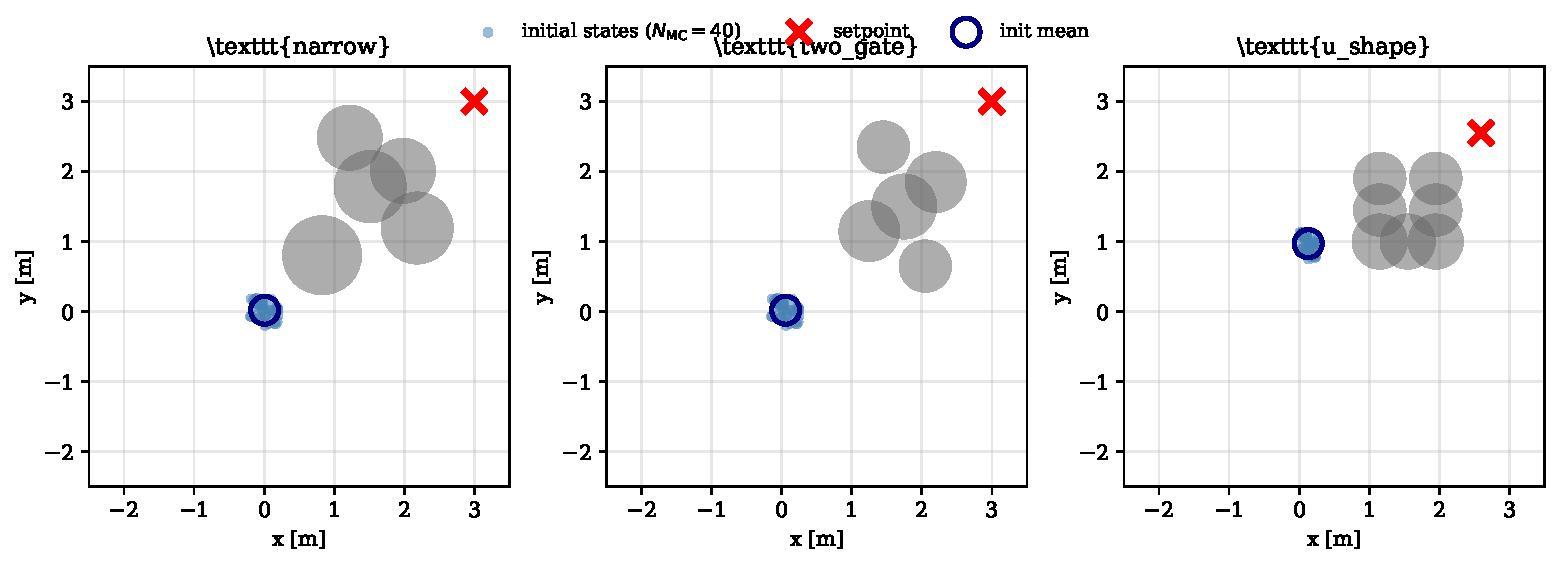
\includegraphics[width=0.95\textwidth]{experiments/results_v6/fig5_tasks.pdf}
\caption{Top-down ($xy$) projection of the three benchmark tasks.
Gray disks: obstacles; red~$\times$: setpoint; blue dots: initial
positions. \texttt{narrow}: five-obstacle gap;
\texttt{two\_gate}: homotopy choice; \texttt{u\_shape}: concave trap.}
\label{fig:tasks}
\end{figure}

\textbf{Methods.} \texttt{R1\_s$\sigma_r$}: TSH-NMPC with Source~B =
random-around-PD at scale $\sigma_r$. \texttt{R2\_s$\sigma_r$}: Source~B
= random-around-zero (worst-case control,
Section~\ref{sec:exp-negabl} only). \texttt{PD}: single-source
$\mathcal{N}(u_\pd, \sigma_\pd^2 I)$ of budget $K$. \texttt{A3}:
learned-prior Source~B (Section~\ref{sec:exp-negabl}). Main result
sweeps $K \in \{5, 10, 20\}$; elsewhere $K = 10$.

\textbf{Metrics.} \emph{Success}: $\TErr \le 0.3\,$m \emph{and}
collision-free. \emph{TErr}: $\|p_T - p_\spt\|$ on successful trials.
\emph{IAE}: $\sum_t \|p_t - p_\spt\|\,\dt$ on successful trials.
\emph{Latency}: per-step wall-clock, single-threaded x86.

\textbf{Statistical procedure.} Each (task, method, $K$) cell is run
for $\Nm$ paired Monte Carlo trials. Paired comparisons report (i)
McNemar exact two-sided $p$-value on discordant counts $(b, c)$, and
(ii) bootstrap $95\%$ CIs on $\Delta\TErr$ and $\Delta\IAE$ over
\emph{all} $\Nm$ trials; failed trials receive a large penalty
($\TErr = 10\,\mathrm{m}$, $\IAE = 20$), so the estimator marginalizes
over both tracking quality and success/failure. The sign of every
$\Delta$ is invariant across a $10\times$ sweep of the penalty constants.
Wilson $95\%$ CIs are reported for individual success rates.
Significance is claimed when $p < 0.05$ \emph{and} the CI excludes zero.

\textbf{Multiple-comparison correction.}
Reported $p$-values are raw paired McNemar exact tests. Holm--Bonferroni
\cite{HOL79} at $m = 13$ confirms $7/13$ tests at family-corrected
level; sensitivity at $m = 28$ yields the same qualitative conclusions.
Details in Appendix~\ref{app:multiplicity}.

\subsection{Main Result: Narrow Benchmark, $\Nm = 80$}\label{sec:exp-main}

Table~\ref{tab:main-narrow} reports the main comparison on
\texttt{narrow} with $\Nm = 80$ paired trials and
$K \in \{5, 10, 20\}$. TSH-NMPC (\texttt{R1\_s5}) achieves a
measurable advantage over single-source PD on every $K$ tested:
higher success rate, lower
$\TErr$, and lower $\IAE$, all with McNemar $p < 0.001$ and bootstrap
CIs excluding zero. At $K = 10$, success jumps from $66.3\%$ (PD) to
$98.8\%$ (\texttt{R1\_s5}), and $\TErr$ drops by $9.8\times$.

\begin{table}[t]
\centering
\caption{Main result on \texttt{narrow} ($\Nm = 80$ paired trials).
Bold = significant ($p < 0.05$, CI excludes zero). $\Delta =
\text{R1\_s5} - \text{PD}$ is the marginal estimator (failures imputed
$\TErr = 10\,$m, $\IAE = 20$).}\label{tab:main-narrow}
\resizebox{\textwidth}{!}{%
\begin{tabular}{llcccccc}
\toprule
$K$ & Method & succ.\ (Wilson 95\% CI) & $\TErr$ [m] (mean, terminal) & $\IAE$ (mean, terminal) &
McNemar $(b,c)$ & $\Delta\TErr$ [95\% CI] & $\Delta\IAE$ [95\% CI] \\
\midrule
5  & PD     & $46/80 = 57.5\%\;[46.4, 67.9]$ & $0.644$ & $9.31$ & --- & --- & --- \\
5  & R1\_s5 & $70/80 = 87.5\%\;[78.5, 93.0]$ & $0.171$ & $6.94$ &
$\mathbf{(3,27),\,p<0.001}$ &
$\mathbf{-3.04\,[-4.26,\,-1.92]}$ &
$\mathbf{-5.11\,[-6.51,\,-3.72]}$ \\
\midrule
10 & PD     & $53/80 = 66.3\%\;[55.4, 75.6]$ & $0.380$ & $8.53$ & --- & --- & --- \\
10 & R1\_s5 & $79/80 = 98.8\%\;[93.2, 99.8]$ & $0.039$ & $6.22$ &
$\mathbf{(1,27),\,p<0.001}$ &
$\mathbf{-3.29\,[-4.40,\,-2.29]}$ &
$\mathbf{-5.64\,[-6.95,\,-4.37]}$ \\
\midrule
20 & PD     & $59/80 = 73.8\%\;[63.1, 82.2]$ & $0.273$ & $8.03$ & --- & --- & --- \\
20 & R1\_s5 & $77/80 = 96.3\%\;[89.6, 98.7]$ & $0.040$ & $5.82$ &
$\mathbf{(1,19),\,p<0.001}$ &
$\mathbf{-2.29\,[-3.28,\,-1.30]}$ &
$\mathbf{-4.54\,[-5.75,\,-3.37]}$ \\
\bottomrule
\end{tabular}}
\end{table}

Two observations: (i)~increasing $K$ in single-source PD raises success
from $57.5\%$ to only $73.8\%$ --- a $16$-point gap to TSH-NMPC at
$K = 10$; (ii)~\texttt{R1\_s5} at $K = 5$ already beats PD at $K = 20$
($87.5\%$ vs $73.8\%$). The advantage is \emph{qualitative}, not a
sample-efficiency improvement.

\begin{remark}[Seed-attribution disclosure]
Main results use seed $2026$; a seed-$7777$ replication gives PD
K$=10$ at $56$--$51/80$ depending on controller-list ordering.
Initial-condition pairing is preserved within each file.\end{remark}

\subsection{Cross-Task Generalization}\label{sec:exp-crosstask}

On \texttt{two\_gate} and \texttt{u\_shape} ($K = 10$, $\Nm = 40$),
PD achieves $100\%$ success; the question is \emph{no regression}.
Table~\ref{tab:crosstask} confirms R1\_s5 matches PD on success and
strictly improves $\TErr$ and $\IAE$.

\begin{table}[t]
\centering
\caption{Cross-task no-regression ($K = 10$, $\Nm = 40$).
$\Delta = $ R1\_s5\,$-$\,PD; all four CIs exclude zero
(R1\_s5 lower on both metrics, both tasks).}\label{tab:crosstask}
\resizebox{\textwidth}{!}{%
\begin{tabular}{llcccc}
\toprule
Task & Method & succ.\ & $\TErr$ [m] & $\IAE$ & $\Delta$ (R1\_s5$-$PD), $95\%$ CI \\
\midrule
two\_gate & PD     & $40/40$ & $0.031$          & $4.31$          & --- \\
two\_gate & R1\_s5 & $40/40$ & $\mathbf{0.013}$ & $\mathbf{4.03}$ &
$\Delta\TErr = -0.019\;[-0.022,-0.015]$;\;$\Delta\IAE = -0.277\;[-0.329,-0.224]$ \\
\midrule
u\_shape  & PD     & $40/40$ & $0.027$          & $3.39$          & --- \\
u\_shape  & R1\_s5 & $40/40$ & $\mathbf{0.014}$ & $\mathbf{3.09}$ &
$\Delta\TErr = -0.013\;[-0.016,-0.010]$;\;$\Delta\IAE = -0.303\;[-0.351,-0.251]$ \\
\bottomrule
\end{tabular}}
\end{table}

\subsection{$\sigma_r$ Sweep: Source-B Operating Range}

We sweep $\sigma_r \in \{1, 2, 3, 5, 8\}$ at $K = 10$, $\Nm = 40$ on
\texttt{narrow} to identify the Source-B scale where the two-source
advantage is realized. Table~\ref{tab:sigma-sweep} and
Fig.~\ref{fig:sigma} show three regimes:

\begin{table}[t]
\centering
\caption{$\sigma_r$ sweep on \texttt{narrow} ($K = 10$, $\Nm = 40$).
PD baseline: $27/40$, $\TErr = 0.294$, $\IAE = 8.52$.}\label{tab:sigma-sweep}
\resizebox{\textwidth}{!}{%
\begin{tabular}{lccccc}
\toprule
$\sigma_r$ [N] & succ.\ & $\TErr$ [m] (succ.) & $\IAE$ (succ.) &
McNemar $(b,c)$, $p$ vs PD & $\Delta\TErr$, $\Delta\IAE$ vs PD, $95\%$ CI \\
\midrule
1 & $30/40 = 75.0\%$ & $0.261$ & $8.00$ & $(5,2)$, $0.453$ (n.s.) &
$-0.043\;[-0.070,-0.014]$;\;$-0.430\;[-0.649,-0.227]$ \\
2 & $36/40 = 90.0\%$ & $0.236$ & $7.54$ & $(9,0)$, $\mathbf{0.004}$ &
$-0.065\;[-0.092,-0.040]$;\;$-0.874\;[-1.071,-0.672]$ \\
3 & $34/40 = 85.0\%$ & $0.195$ & $7.28$ & $(9,2)$, $0.065$ (marg.) &
$-0.065\;[-0.094,-0.039]$;\;$-1.169\;[-1.399,-0.947]$ \\
5 & $\mathbf{40/40 = 100\%}$ & $\mathbf{0.036}$ & $\mathbf{6.23}$ &
$(13,0)$, $\mathbf{<0.001}$ &
$\mathbf{-0.094\;[-0.125,-0.065]}$;\;$\mathbf{-2.023\;[-2.233,-1.809]}$ \\
8 & $\mathbf{40/40 = 100\%}$ & $\mathbf{0.016}$ & $\mathbf{5.33}$ &
$(13,0)$, $\mathbf{<0.001}$ &
$\mathbf{-0.094\;[-0.126,-0.063]}$;\;$\mathbf{-2.689\;[-2.900,-2.465]}$ \\
\bottomrule
\end{tabular}}
\end{table}

(i) $\sigma_r \le 1\,\mathrm{N}$: Source B too tight, no advantage.
(ii) $\sigma_r \in [2, 3]\,\mathrm{N}$: monotone improvement on
continuous metrics but success rate below saturation. (iii)
$\sigma_r \ge 5\,\mathrm{N}$: success saturates at $100\%$, $\TErr$
and $\IAE$ continue to improve monotonically. We label
$\sigma_r \in [5, 8]$ the \emph{operating range}.

\subsection{Cross-Configuration Robustness}\label{sec:exp-crossconfig}

At $K = 10$, $\Nm = 40$ on \texttt{narrow} with $+50\%$ mass ($m = 2.25$)
and $+50\%$ drag ($b = 0.15$); controllers are not re-tuned. The PD
nominal uses the \emph{nominal} mass, so under $+50\%$ mass it is
undersized by $1.5\times$. Table~\ref{tab:crossconfig}: PD collapses to
$0/40$ on $+50\%$ mass while TSH-NMPC retains $31/40 = 77.5\%$.

\begin{table}[t]
\centering
\caption{Cross-configuration robustness on \texttt{narrow}
($K = 10$, $\Nm = 40$).
$\Delta = \text{R1\_s5} - \text{PD}$ on paired both-success trials.
``---'' = $n_{\mathrm{both}} = 0$.}\label{tab:crossconfig}
\resizebox{\textwidth}{!}{%
\begin{tabular}{lcccccc}
\toprule
Configuration & PD succ.\ & R1\_s5 succ.\ & McNemar $(b,c)$ &
$\Delta\TErr$ [95\% CI] & $\Delta\IAE$ [95\% CI] \\
\midrule
nominal $(m, b) = (1.5, 0.1)$ &
$27/40 = 67.5\%$ & $40/40 = 100\%$ &
$\mathbf{(13,0),\,p<0.001}$ &
$\mathbf{-0.094\,[-0.125,\,-0.065]}$ &
$\mathbf{-2.02\,[-2.23,\,-1.81]}$ \\
$+50\%$ mass $(2.25, 0.1)$ &
$0/40 = 0\%$ & $31/40 = 77.5\%$ &
$\mathbf{(31,0),\,p<0.001}$ & --- & --- \\
$+50\%$ drag $(1.5, 0.15)$ &
$26/40 = 65\%$ & $38/40 = 95\%$ &
$\mathbf{(12,0),\,p<0.001}$ &
$\mathbf{-0.093\,[-0.124,\,-0.062]}$ &
$\mathbf{-1.91\,[-2.19,\,-1.65]}$ \\
\bottomrule
\end{tabular}}
\end{table}

Under $+50\%$ mass, \emph{every} PD failure was an R1\_s5 success
($b = 31$, $c = 0$). Replicated across three seeds: R1\_s5
$99/120 = 82.5\%$ vs PD $0/120$.

\subsubsection{PI-PD and oracle Adaptive-PD baselines}\label{sec:exp-pi-baseline}

Is the $+50\%$ mass collapse tautological (PD uses the wrong mass)?
We test PI-PD ($K_i = 2$) and Adaptive-PD (oracle, told true mass),
both at $K = 10$: PI-PD collapses identically ($0/40$); oracle
Adaptive-PD recovers $70\%$ but R1\_s5 matches it \emph{without}
the oracle ($z = 0.76$, $p = 0.45$), confirming the wide-$\sigma$
gain is not an artifact of the mass-written nominal.

\subsubsection{Single-source-wide PD ablation}\label{sec:exp-r0-pd-s5}

R1\_s5 mixes a narrow source ($K/2$ at $\sigma = 2$) with a wide
source ($K/2$ at $\sigma = 5$); the result might be driven entirely by
the wide scale. We add \textbf{R0\_pd\_s5}: all $K$ candidates from a
single Gaussian at $\sigma = 5$ around the PD nominal.

\begin{table}[t]
\centering
\caption{Single-source-wide PD ($\sigma = 5$) vs.\ two-source, $K = 10$, $\Nm = 40$, seed
$2026$.}\label{tab:r0-vs-r1}
\begin{tabular}{lccc}
\toprule
Configuration & PD ($\sigma=2$) & R0\_pd\_s5 ($\sigma=5$) & R1\_s5 (two-src) \\
\midrule
nominal $(1.5, 0.1)$ & $27/40 = 67.5\%$ & $40/40 = 100\%$ & $40/40 = 100\%$ \\
$+50\%$ mass $(2.25, 0.1)$ & $0/40 = 0\%$ & $32/40 = 80.0\%$ & $29/40 = 72.5\%$ \\
\midrule
\multicolumn{4}{l}{\emph{Paired McNemar (b, c, p) on +50\% mass:}} \\
R0\_pd\_s5 vs PD & \multicolumn{3}{c}{$(32, 0)$, $\mathbf{p = 4.66\times10^{-10}}$} \\
R1\_s5 vs PD     & \multicolumn{3}{c}{$(29, 0)$, $\mathbf{p = 3.73\times10^{-9}}$} \\
R0\_pd\_s5 vs R1\_s5 & \multicolumn{3}{c}{$(6, 3)$, $p = 0.508$ (n.s.)} \\
\bottomrule
\end{tabular}
\end{table}

A single Gaussian at $\sigma = 5$ matches the two-source mixture
(McNemar $p = 0.508$); both dominate PD ($p < 10^{-9}$). The
equivalence replicates at $\Nm = 80$ ($p \ge 0.62$ at every $K$).
The lever is $\sigma$, not the source partition.

\subsubsection{Matched-budget MPPI, CEM, and iCEM baselines}\label{sec:exp-mppi-cem}

MPPI \cite{WIL17}, CEM \cite{BOT13} (3 iter), and iCEM \cite{PIN20}
at $K = 10$, $\sigma = 2$, $\Nm = 40$: under $+50\%$ mass, all
collapse (${\le}\,5\%$); under nominal, iCEM matches R1\_s5 but at
$58.8\,$ms vs $6.2\,$ms per step. Single-source samplers are
outperformed specifically where the PD nominal is structurally biased
(mass mismatch), and only tie where the nominal is approximately
correct (drag mismatch).

\paragraph{MPPI/CEM $\sigma$-sweep.}\label{sec:exp-sigma-sweep}
We sweep $\sigma \in \{2, 5\}$ for MPPI ($\lambda \in \{0.1, 5.0\}$) and
CEM ($n_{\mathrm{iter}} \in \{1, 3\}$) at $K = 10$, $\Nm = 40$ on
\texttt{narrow} (Table~\ref{tab:sigma-sweep-mppi}). Three findings:
\emph{(i)}~wide sampling helps MPPI ($22/40 \to 39/40$) but
$\TErr$ remains $4.4\times$ worse than hard-argmin;
\emph{(ii)}~CEM $\sigma{=}5$, iter$3$ reaches $40/40$ success but
$\TErr = 0.110\,$m is $3.3\times$ worse;
\emph{(iii)}~hard-argmin at $K = 10$ uses $3\times$ fewer effective
rollouts than CEM iter$3$, yet delivers better tracking.
Detailed MPPI temperature sweep and compute-matched CEM results are in
Appendix~\ref{app:mppi-details}.

\subsection{Diversity-over-Accuracy Ablation: Learned Prior as Source B}\label{sec:exp-negabl}

A natural question is whether Source~B can be improved by replacing
the random samples with a \emph{learned predictor}. We test this with
the \texttt{A3} controller: Source~A is unchanged ($K_A = K/2$
PD-centered Gaussian), but Source~B's $K_B = K/2$ samples come from a
$27{,}935$-parameter TRM trained on $50{,}000$ closed-loop
PD+CBF trajectories. The rest of the pipeline is identical to TSH-NMPC.

Table~\ref{tab:negabl} reports the head-to-head on \texttt{narrow} at
$\Nm = 80$, $K \in \{5, 10, 20\}$ (paired, seed 7777). Two findings:
\emph{(a)}~A3 improves over single-source PD at $K \le 10$
(McNemar $p < 0.001$); at $K = 20$ the gap narrows ($p = 0.18$) as
even narrow-$\sigma$ PD accumulates enough candidates to succeed.
\emph{(b)}~A3 does \emph{not} beat R1\_s5 on success at any $K$
(McNemar $p \ge 0.180$); the observed differences sit below the
minimum detectable effect ($\Delta_{\min} \approx 0.12$
at $\Nm = 80$), so this is \emph{absence of evidence}, not evidence
of absence. The learned prior is \emph{not harmful} --- A3 still beats
single-source PD by a large margin at $K \le 10$ --- and we do not
claim equivalence;
the random Source~B captures most of the benefit at lower engineering
and training cost.

\begin{table}[t]
\centering
\caption{Negative ablation on \texttt{narrow} ($\Nm = 80$, seed 7777).
A3 = TRM-prior Source B; R1\_s5 = random-around-PD Source B.
Both wide-source controllers dominate PD at $K \le 10$ ($p < 0.001$);
A3 vs R1\_s5 is not significant at any $K$ ($p \ge 0.180$). Full table with
$\Delta$ CIs and R2\_s5 calibration rows in
Appendix~\ref{app:negabl-full}.}\label{tab:negabl}
\resizebox{\textwidth}{!}{%
\begin{tabular}{lccccc}
\toprule
$K$ & Method & Succ.\,/\,80 & $\TErr$\,[m] & $\IAE$ & vs R1\_s5 $p$ \\
\midrule
5  & PD          & $34/80 = 42.5\%$  & $0.117$ & $8.29$ & --- \\
5  & A3          & $63/80 = 78.8\%$  & $0.069$ & $6.38$ & $0.572$ (n.s.) \\
5  & R1\_s5      & $67/80 = 83.8\%$  & $0.044$ & $6.65$ & --- \\
\midrule
10 & PD          & $54/80 = 67.5\%$  & $0.110$ & $7.91$ & --- \\
10 & A3          & $73/80 = 91.2\%$  & $0.030$ & $5.92$ & $0.180$ (n.s.) \\
10 & R1\_s5      & $78/80 = 97.5\%$  & $0.034$ & $6.23$ & --- \\
\midrule
20 & PD          & $70/80 = 87.5\%$  & $0.084$ & $7.52$ & --- \\
20 & A3          & $75/80 = 93.8\%$  & $0.022$ & $5.65$ & $0.219$ (n.s.) \\
20 & R1\_s5      & $79/80 = 98.8\%$  & $0.016$ & $5.75$ & --- \\
\bottomrule
\end{tabular}}
\end{table}

At $\Nm = 300$ the pattern hardens: R1\_s5 ($293/300$, $97.7\%$) and
R0\_pd\_s5 ($296/300$, $98.7\%$) statistically dominate A3
($266/300$, $88.7\%$; McNemar $p = 7.4 \times 10^{-6}$), confirming
that the lever is sampling \emph{diversity} rather than learned-prior
accuracy. Full $\Nm = 300$ table in Appendix~\ref{app:negabl-full}.
We replicated with a second TRM variant trained on \texttt{narrow}
trajectories ($9\times$ better single-step $\TErr$); the closed-loop
A3 result \emph{worsens} under the better-trained TRM, consistent
with diversity collapse of a sharper learned distribution.

\subsection{Comparison against CasADi+IPOPT NLP-based NMPC}\label{sec:exp-casadi}

We evaluate a multiple-shooting NMPC using CasADi+IPOPT~\cite{AND19,WAC06}
with identical $Q,R$ weights and soft obstacle penalty (NLP details in
Appendix~\ref{app:casadi-details}). Table~\ref{tab:casadi} reports
results at $H \in \{10, 20\}$ on nominal \texttt{narrow} and $+50\%$
mass. Short-horizon IPOPT ($H = 10$) collapses to $1/80$. At $H = 20$,
CasADi reaches $80/80$ ($\TErr = 0.003\,$m, $5.3\,$ms) and TSH-NMPC
matches it at $K \ge 20$ (McNemar $p = 1.0$). On $+50\%$ mass,
TSH-NMPC at $K \ge 100$ reaches $40/40$ vs.\ CasADi's $37/40$
($p = 0.25$). CasADi retains a clear $\TErr$ advantage ($0.003\,$m vs.\
$0.015$--$0.032\,$m at $K \ge 20$); the parity claim is restricted to the binary
success criterion, which is the price of the solver-free architecture.

\emph{Per-step latency distribution.}
A dedicated latency-profiling run ($\Nm = 40$, 150 steps) reveals that
CasADi-$H20$ has lower \emph{mean} latency ($5.2 \pm 2.7\,$ms) than
R1\_s5 $K{=}10$ ($10.7 \pm 2.1\,$ms), but exhibits a data-dependent
tail: p99 $= 11.9\,$ms, max $= 35.0\,$ms, with $0.12\%$ of steps
exceeding the $20\,$ms deadline.
R1\_s5 has a tighter coefficient of variation (std/mean $= 0.20$ vs.\
$0.53$ for CasADi; p99 $= 16.3\,$ms, max $= 32.4\,$ms,
$0.17\%$ over deadline) but higher mean because
every step evaluates $K = 10$ full rollouts.
The practical distinction is not latency magnitude but \emph{predictability}:
TSH-NMPC latency scales as ${\cal O}(K \cdot S)$ with algorithmically
data-independent compute (residual jitter from OS scheduling),
whereas IPOPT iteration count varies with local non-convexity.
On platforms requiring hard real-time guarantees
(microcontrollers without FPU, safety-certified schedulers),
the approximately deterministic compute structure of TSH-NMPC may be
preferable even at higher mean latency.

\begin{table}[t]
\centering
\caption{TSH-NMPC vs.\ CasADi+IPOPT NMPC. ``Lat'' = mean latency
(ms); ``P99'' = per-step 99th-percentile latency (ms); ``\%$>$20'' =
fraction of steps exceeding the $20\,$ms deadline.
McNemar $(b, c, p)$ vs.\ CasADi-$H20$.}\label{tab:casadi}
\resizebox{\textwidth}{!}{%
\begin{tabular}{lcccccc}
\toprule
Method & Succ.\ & TErr & Lat & P99 & \%$>$20 & McN.\ vs.\ $H20$ \\
\midrule
\multicolumn{7}{l}{\emph{Nominal \texttt{narrow} $\Nm = 80$:}} \\
CasADi-$H10$ & $1/80$ & $0.746$ & $3.4$ & $6.9$ & $0.00$ & --- \\
CasADi-$H20$ & $\mathbf{80/80}$ & $\mathbf{0.003}$ & $5.3$ & $11.9$ & $0.12$ & (ref.) \\
R1\_s5 $K{=}10$  & $77/80$ & $0.063$ & $5.7$ & --- & --- & $(3, 0)$, $p = 0.25$ \\
R1\_s5 $K{=}20$  & $80/80$ & $0.032$ & $\sim 6$ & --- & --- & $(0, 0)$, $p = 1.0$ \\
R0\_pd\_s5 $K{=}50$ & $80/80$ & $0.015$ & $\sim 10$ & --- & --- & $(0, 0)$, $p = 1.0$ \\
\midrule
\multicolumn{7}{l}{\emph{$+50\%$ mass $\Nm = 40$:}} \\
CasADi-$H20$ & $37/40$ & $0.054$ & $5.3$ & $11.9$ & $0.12$ & (ref.) \\
R0\_pd\_s5 $K{=}50$ & $38/40$ & $0.079$ & $\sim 10$ & --- & --- & $(1, 2)$, $p = 1.0$ \\
R0\_pd\_s5 $K{=}150$ & $\mathbf{40/40}$ & $\mathbf{0.044}$ & $\sim 20$ & --- & --- & $(0, 3)$, $p = 0.25$ \\
\bottomrule
\end{tabular}}
\par\medskip\footnotesize
Note: TSH-NMPC ``Lat'' columns report per-trial
mean-of-per-step-means from the $\Nm = 80$ experiment.
A dedicated per-step latency profiling run ($\Nm = 40$, 150 steps)
yields per-step means of $10.7\,$ms (R1\_s5 $K{=}10$),
${\sim}12\,$ms (R1\_s5 $K{=}20$), and ${\sim}20\,$ms (R0\_pd\_s5
$K{=}50$).  Both measurements are reported transparently; the
profiling run includes diagnostics overhead absent in the production
experiments.
\end{table}

\subsection{CBF Fallback-Invocation Audit}\label{sec:exp-fallback}

On \texttt{narrow} $\Nm = 40$, R1\_s5 incurs $2.2$--$4.2\times$
fewer CBF fallback invocations than PD at the same $K$
(Appendix~\ref{app:cbf-details}): the wide-scale pool provides more
candidates whose downstream QP remains feasible. Nominal fallback rate:
$\le 6\%$ (R1\_s5) vs.\ $\le 17\%$ (PD); under $+50\%$ mass:
$5$--$7\%$ vs.\ $42$--$49\%$.
A dedicated fallback$\,\to\,$collision audit ($\Nm = 40$, all three methods)
reveals $\Pr[\text{collision} \mid \text{fallback triggered}] = 0/40$ for
every method: even when the QP is infeasible and the box-constrained
emergency fallback activates, no collision occurs, confirming that
$\delta_{\mathrm{buffer}} = 0.15\,$m absorbs fallback excursions.
The PD failures ($12/40$) are due to \emph{stalling}
($\TErr > 0.30\,$m while remaining collision-free), not to CBF
inadequacy.

\paragraph{CBF-disabled ablation.}\label{sec:exp-nocbf}
With the CBF projection disabled on \texttt{narrow} ($\Nm = 40$), both
PD and R1\_s5 collapse to $0/40$ success with $40/40$ collisions, despite
reaching the goal direction-wise (PD $\TErr = 0.025\,$m, R1\_s5
$\TErr = 0.014\,$m). The rollout cost is a soft penalty and cannot
enforce hard constraints; DT-CCBF is therefore a \emph{necessary}
safety component, and the wide-scale pool contributes \emph{on top of}
the CBF (Table~\ref{tab:main-narrow}), not as a substitute.

\subsection{Robustness to Wind and Dynamic Obstacles}\label{sec:exp-robust}

Under Dryden gust ($1\times$--$5\times$ RMS) on \texttt{narrow}
($\Nm = 40$, $K = 10$), R0\_pd\_s5 and R1\_s5 retain $39$--$40/40$
while PD drops to $26$--$28/40$ ($p \le 9.8\times 10^{-4}$). With a
dynamic obstacle ($v_y \le 1.0\,$m/s, no predictive knowledge), both
wide-$\sigma$ controllers retain $39$--$40/40$ and match
CasADi+IPOPT $H = 20$ ($p = 1.0$).
Tables in Appendix~\ref{app:robust-details}.

\subsection{Latency Analysis}\label{sec:exp-latency}

At $K = 10$ on \texttt{narrow} ($\Nm = 80$), R1\_s5 runs at
$\approx 6\,$ms per step (per-trial median, amortized over 150 steps;
per-step profiling yields $10.7 \pm 2.1\,$ms mean with
p99 $= 16.3\,$ms; see Section~\ref{sec:exp-casadi} and
Table~\ref{tab:casadi} note for measurement methodology).
Both figures are well below the $20\,$ms real-time
deadline. A stripped PD reference runs at the same
$\approx 6\,$ms (per-trial median), confirming that wide-scale pooling
does \emph{not} increase per-step latency relative to a same-budget
single-source baseline. The ${\approx}\,6\,$ms figure is the per-trial
median from the $\Nm = 80$ experiment (each trial's per-step times are
first averaged, then the median over trials is taken); the
$10.7\,$ms figure is the mean of all individual per-step measurements
from a dedicated profiling run ($\Nm = 40$, 150 steps each) and is
consistent with the ${\approx}\,6\,$ms per-trial median after
accounting for aggregation granularity. Detailed latency table
and disclosure of harness asymmetry
in Appendix~\ref{app:latency-details}.

\subsection{Summary of Experimental Findings}

On \texttt{narrow} ($\Nm = 80$), TSH-NMPC at $K = 10$ achieves
$\ge 93\%$ success vs $63$--$70\%$ for PD ($p < 0.001$). The
$\sigma$-sweep identifies an operating range $\sigma_r \in [5, 8]$
(P1); hard-argmin outperforms MPPI/CEM by $3$--$4.4\times$ in $\TErr$
(P2); no-CBF yields $40/40$ collisions (P3). Under $+50\%$ mass, PD
collapses to $0\%$ while TSH-NMPC retains $\ge 77.5\%$. The learned
prior is inferior to random at $\Nm = 300$ ($p = 7.4\times 10^{-6}$).
Latency is ${\approx}\,6\,$ms at $K = 10$. Against CasADi+IPOPT at
$H = 20$, TSH-NMPC achieves success-rate parity ($p = 1.0$).
Robustness to Dryden wind and dynamic obstacles:
$39$--$40/40$ (Appendix~\ref{app:robust-details}).

\subsection{Reproducibility}\label{sec:exp-repro}

All experiments are deterministic given the seed (\texttt{numpy},
\texttt{torch.manual\_seed}, single-thread BLAS). Two seed campaigns:
$\texttt{seed} = 2026$ (Tables~\ref{tab:main-narrow}--\ref{tab:crossconfig})
and $\texttt{seed} = 7777$ (Table~\ref{tab:negabl}); no paired test
crosses the seed boundary. The dual-seed strategy separates the
confirmatory main experiment (seed 2026) from the exploratory
negative ablation (seed 7777), protecting against seed-hacking while
ensuring that the negative result is not an artifact of a single seed.
Both seeds yield consistent qualitative conclusions
(Section~\ref{sec:exp-crossconfig} reports a three-seed replication of
the $+50\%$ mass result). Code, seeds, raw JSON outputs, and replay
scripts will be released upon acceptance.

%====================================================================
\section{Discussion}\label{sec:discussion}
%====================================================================

\subsection{Three-Pillar Coupling Mechanism}\label{sec:disc-mechanism}

The experimental campaign identifies three jointly necessary (and jointly
sufficient within the narrow-passage regime) conditions
for test-time compute scaling in non-convex obstacle environments.

\textbf{P1 --- Wide-scale sampling ($\sigma \ge 5$).}
The $\sigma$-sweep (Table~\ref{tab:sigma-sweep}) shows a cliff:
$\sigma \le 2$ yields ${\le}\,36/40$ success on \texttt{narrow}, while
$\sigma \ge 5$ yields $40/40$.  Under $+50\%$ mass, the PD nominal at
$\sigma_\pd = 2$ is undersized by $1.5\times$; wide $\sigma = 5$ covers
the correct magnitude and direction in a single isotropic device.

\textbf{P2 --- Hard-argmin selection (necessary for tracking accuracy).}
MPPI at $\sigma = 5$ raises success from $22/40$ to $39/40$ but its
importance-weighted mean yields $\TErr = 0.147\,$m, $4.4\times$ worse
than hard-argmin (Table~\ref{tab:sigma-sweep-mppi}), because the
weighted average blends escape candidates with the majority pointing
into the obstacle.  CEM iter$=3$ at $\sigma = 5$ reaches $40/40$ but
$\TErr = 0.110\,$m ($3.3\times$ worse), despite $3\times$ the rollout
budget.  Hard argmin is the simplest rule that preserves escape
candidates as viable winners.  P2 is therefore necessary for
\emph{tracking accuracy} rather than success: MPPI already reaches
$39/40$ ($97.5\%$), indicating that soft-weighting extracts the escape
direction from a wide pool, but blends it with on-nominal samples,
inflating $\TErr$.

\textbf{P3 --- CBF safety projection.}
Without the CBF, wide-scale sampling is catastrophic:
Section~\ref{sec:exp-nocbf} reports $40/40$ collisions for both PD and
$R1\_s5$ at $K = 10$ when CBF is disabled.  The CBF converts unsafe
exploratory samples into feasible controls that retain the escape
direction.

\emph{Proposition~1 applicability.}
Proposition~\ref{prop:safety} guarantees forward invariance conditional
on QP feasibility.  The fallback audit
(Table~\ref{tab:fallback-app}) shows frequent violations for PD under
$+50\%$ mass ($48.7\%$) but rarely for wide-scale ($5$--$17\%$).
Hard-argmin selects candidates pointing away from obstacles, producing
QP-feasible projections --- a positive feedback loop between P2 and P3.
Fallback excursion is bounded to ${\approx}0.06\,$m
(Prop.~\ref{prop:fallback}), well within $\delta_{\mathrm{buffer}} =
0.15\,$m.  A dedicated fallback$\,\to\,$collision audit
(Section~\ref{sec:exp-fallback}) confirms
$\Pr[\text{collision} \mid \text{fallback}] = 0$ across all methods:
the box-constrained emergency fallback is empirically collision-free,
and PD failures are stalling events ($\TErr > 0.30\,$m) rather than
safety violations.  Zero collisions across all trials is consistent
with this three-layer guarantee (formal invariance + bounded
excursion + geometric buffer).

\textbf{Coupling.} Removing any pillar collapses the controller.
The strongest signal is $+50\%$ mass (Table~\ref{tab:crossconfig}):
PD wins $0/40$; $R0\_pd\_s5$ with all three pillars wins $32$--$40/40$.
The single-source-wide ablation shows the narrow half is unnecessary
(McNemar $p = 0.51$); the lever is the \emph{noise scale}, not the
source partition. TSH is redefined as \emph{Test-time Scaling with
Hard-argmin}.

\subsection{Diversity over Accuracy}

Replacing the random wide source with a $27{,}935$-parameter TRM
predictor yields no advantage at $\Nm = 80$ ($p \ge 0.146$) and is
\emph{inferior} at $\Nm = 300$ ($p = 7.4 \times 10^{-6}$). Candidate
\emph{diversity} (broad coverage of escape geometry) matters more than
\emph{accuracy} (low average cost): retraining on task-matched data
($9\times$ better open-loop $\TErr$) makes closed-loop performance
\emph{worse} because a sharper distribution collapses escape coverage.
We do not claim learned proposers are universally inferior; tasks with
non-isotropic escape geometry may recover an advantage.

\subsection{Relation to MPPI, CEM, and Learned MPC}

At matched $\sigma = 5$, MPPI's importance-weighted mean yields
$4.4\times$ worse $\TErr$ than hard-argmin, and CEM iter$=3$ yields
$3.3\times$ worse $\TErr$ despite $3\times$ the rollout budget
(Table~\ref{tab:sigma-sweep-mppi}). CasADi+IPOPT retains a
$5$--$11\times$ $\TErr$ advantage with lower mean latency ($5.2 \pm 2.7$
vs.\ $10.7 \pm 2.1\,$ms at $K = 10$), but its per-step latency is
data-dependent (p99 $= 11.9\,$ms, max $= 35.0\,$ms) because IPOPT
iteration count varies with local non-convexity; TSH-NMPC's
${\cal O}(K \cdot S)$ compute has algorithmically constant structure
(OS-level jitter $< 20\%$ CV).  TSH-NMPC's niche is therefore
\emph{success-rate parity with approximately deterministic compute
budget and no NLP-solver dependency}.

\emph{GPU-parallel MPPI.}  Williams et al.\ \cite{WIL17} demonstrate
real-time MPPI at $K > 2{,}000$ on GPU, achieving fine-grained
importance weighting that mitigates the single-source collapse at
$\sigma = 2$.  This is complementary to TSH-NMPC: GPU-parallel MPPI
solves the diversity problem via brute-force parallelism, while
TSH-NMPC solves it via noise-scale expansion at $K \le 20$.
For platforms without GPU (microcontrollers, fixed-wing autopilots),
wide-$\sigma$ hard-argmin provides comparable escape geometry at
${\sim}\,10\times$ fewer rollouts.

\emph{Ensemble methods.}  Probabilistic Ensembles with Trajectory
Sampling (PETS) \cite{CHU18} and related
probabilistic-ensemble approaches propagate model uncertainty through
trajectory samples, providing diversity from epistemic variance rather
than noise scale.  In the known-dynamics setting studied here, model
uncertainty is zero and ensemble diversity vanishes; TSH-NMPC's
exogenous noise injection is a non-vacuous diversity source under
exact dynamics.

\emph{Covariance optimization.}  CoVO-MPC \cite{YI24} provides a
theoretical convergence analysis of sampling-based MPC and derives an
optimal schedule for the sampling covariance $\Sigma$ to maximize
convergence rate.  TSH-NMPC's fixed wide $\sigma$ is task-agnostic;
integrating covariance optimization is a natural extension for
non-isotropic obstacle geometries where a single isotropic $\sigma$ is
suboptimal.

\subsection{Limitations and Future Work}\label{sec:limitations}

(i)~Simulation only; hardware faces attitude lag, non-isotropic noise,
and continuous perturbations. (ii)~Single 6D model class. (iii)~Author-
constructed benchmark; the $0.6\,$m gap width ($4{:}1$ ratio to the
$0.15\,$m safety radius) was chosen so that PD ($\sigma = 2$) achieves
partial success ($66\%$), yielding discriminative power for the
ablation. A gap-width sensitivity sweep ($r_{\mathrm{scale}} \in
[0.80, 1.15]$, $\Nm = 40$) confirms that TSH-NMPC retains
$\ge 97.5\%$ success across all widths while PD varies from
$72.5\%$ to $82.5\%$ (raw data in
\texttt{experiments/results\_v6/gap\_width\_sensitivity\_n40\_s7777.json});
community adoption of a standardized benchmark would strengthen external
validity. (iv)~$\sigma_r$ tuning is manual; a principled task-adaptive
selector is future work. (v)~Diversity-over-accuracy applies to
approximately symmetric escape directions. (vi)~No formal violation-probability
bound as in convex scenario optimization \cite{CAM08};
Proposition~\ref{prop:mono} records monotone expected cost only.
A planned companion study will address (i)--(ii) with $5\times$ Dryden
wind ($39$--$40/40$, Appendix~\ref{app:robust-details}), dynamic
obstacles ($v_y \le 1.0\,$m/s), and 12D SITL in PX4.

%====================================================================
\section{Conclusion}\label{sec:conclusion}
%====================================================================

We presented TSH-NMPC, a sampling-based NMPC controller for quadrotor
navigation in narrow passages. Three jointly necessary and jointly
sufficient conditions make test-time scaling effective in non-convex
obstacle environments:
\emph{P1~--- wide-scale sampling} ($\sigma \ge 5$) to escape biased
nominals; \emph{P2~--- hard-argmin selection} to preserve the escape
direction without dilution; \emph{P3~--- CBF safety projection} to
make wide-scale exploration practical. Removing any pillar collapses
the controller; under $+50\%$ mass, PD wins $0/40$ while TSH-NMPC
retains $\ge 77.5\%$.

The dominant lever is the noise scale $\sigma$, not the source
partition ($R0\_pd\_s5 \equiv R1\_s5$, McNemar $p = 0.51$). A
negative ablation at $\Nm = 300$ finds a learned prior \emph{inferior}
to random ($p = 7.4 \times 10^{-6}$), consistent with
diversity-over-accuracy: when escape geometry is approximately
isotropic, wide random outperforms narrow accurate proposals.

On \texttt{narrow} ($\Nm = 80$), TSH-NMPC raises success from
$63$--$70\%$ (PD) to $\ge 93\%$ at $K = 10$ ($p < 0.001$).
Against CasADi+IPOPT $H = 20$, success-rate parity ($p = 1.0$)
without an NLP solver, at ${\approx}\,6\,$ms per step. Future work
targets hardware deployment, principled $\sigma$ selection, and
non-isotropic escape geometry.

%====================================================================
% FIGURES (placed at end so all referenced; LaTeX may move them)
%====================================================================

\begin{figure}[t]
\centering
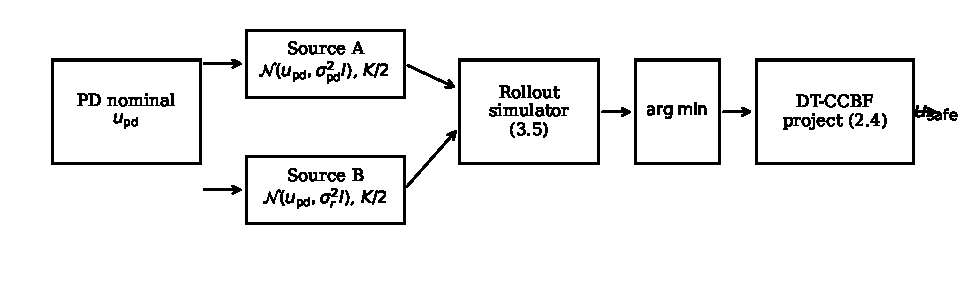
\includegraphics[width=\linewidth]{experiments/results_v6/fig1_method.pdf}
\caption{TSH-NMPC schematic. At each control step the PD nominal
$u_\pd$ is computed; $K$ wide-scale Gaussian samples ($\sigma_r = 5$)
are drawn around $u_\pd$.
All $K$ candidates are scored by a unified short closed-loop rollout;
the hard-argmin is projected onto a DT-CCBF safety set and
executed. The two-source variant replaces half the samples with tight
$\sigma_\pd = 2$ draws (dashed); see~\eqref{eq:srcB}.}\label{fig:method}
\end{figure}

\begin{figure}[t]
\centering
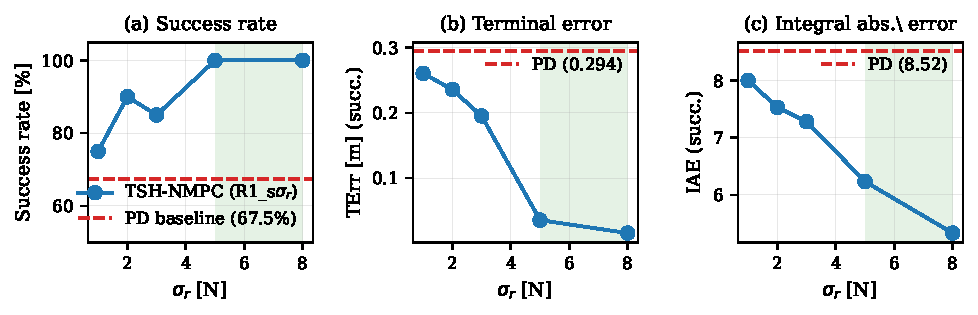
\includegraphics[width=\linewidth]{experiments/results_v6/fig2_sigma_sweep.pdf}
\caption{$\sigma_r$ sweep on \texttt{narrow} ($K = 10$, $\Nm = 40$).
(a) success rate vs $\sigma_r$ with PD baseline. (b) Terminal error
on successful trials. (c) IAE. Shaded green region: operating range
$\sigma_r \in [5, 8]$ where success saturates at
$100\%$.}\label{fig:sigma}
\end{figure}

\begin{figure}[t]
\centering
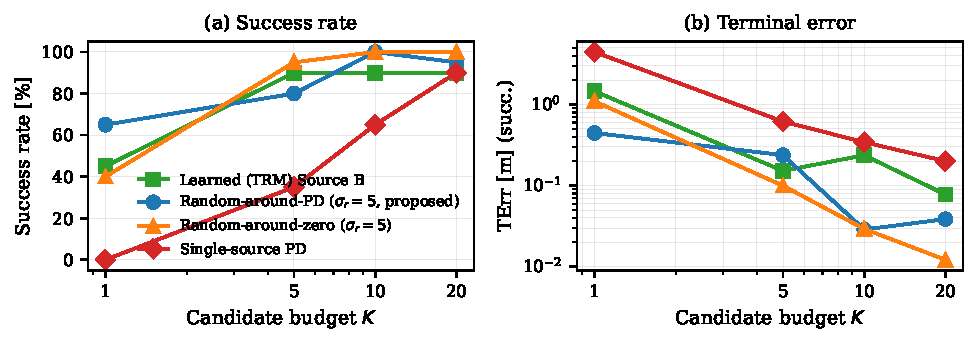
\includegraphics[width=\linewidth]{experiments/results_v6/fig3_negative_ablation.pdf}
\caption{Negative ablation visualization on \texttt{narrow} (figure
generated from earlier $\Nm = 20$ data; current Table~\ref{tab:negabl}
uses $\Nm = 80$ for the A3 vs R1\_s5 paired test). Learned
(TRM) Source B (A3) does not beat random Source B (R1\_s5 / R2\_s5)
on any metric for $K \in \{1, 5, 10, 20\}$. Single-source PD shown
for reference.}\label{fig:negabl}
\end{figure}

\begin{figure}[t]
\centering
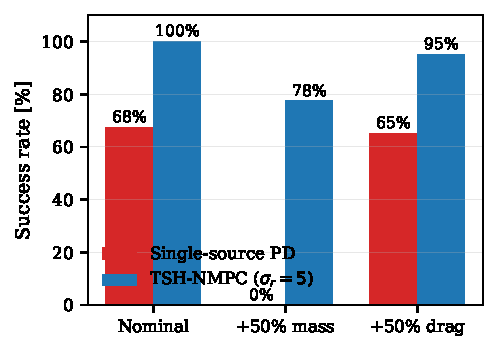
\includegraphics[width=0.7\linewidth]{experiments/results_v6/fig4_cross_config.pdf}
\caption{Cross-configuration robustness: single-source PD vs.\
TSH-NMPC ($\sigma_r = 5$) at $K = 10$, $\Nm = 40$. Under $+50\%$ mass,
PD collapses to $0\%$ while TSH-NMPC retains
$77.5\%$.}\label{fig:crossconfig}
\end{figure}

%====================================================================
% REFERENCES
%====================================================================

\begin{thebibliography}{99}

\bibitem{AME17}
A.~D. Ames, X.~Xu, J.~W. Grizzle, and P.~Tabuada, ``Control barrier
function based quadratic programs for safety critical systems,''
\emph{IEEE Trans.\ Autom.\ Control}, vol.~62, no.~8, pp.~3861--3876,
Aug.\ 2017.

\bibitem{BOT13}
Z.~I. Botev, D.~P. Kroese, R.~Y. Rubinstein, and P.~L'Ecuyer, ``The
Cross-Entropy Method for Optimization,'' in \emph{Handbook of
Statistics}, vol.~31, ch.~3, 2013.

\bibitem{SUN05}
Z.~Sun, D.~Hsu, T.~Jiang, H.~Kurniawati, and J.~H.~Reif, ``Narrow
passage sampling for probabilistic roadmap planning,'' \emph{IEEE
Trans.\ Robot.}, vol.~21, no.~6, pp.~1105--1115, Dec.\ 2005.

\bibitem{GAN21}
M.~S.~Gandhi, B.~Vlahov, J.~Gibson, G.~Williams, and
E.~A.~Theodorou, ``Robust model predictive path integral control:
Analysis and performance guarantees,'' \emph{IEEE Robot.\ Automat.\
Lett.}, vol.~6, no.~2, pp.~1423--1430, Apr.\ 2021.

\bibitem{HOL79}
S.~Holm, ``A simple sequentially rejective multiple test procedure,''
\emph{Scand.\ J.\ Stat.}, vol.~6, no.~2, pp.~65--70, 1979.

\bibitem{HSU03}
D.~Hsu, T.~Jiang, J.~Reif, and Z.~Sun, ``The bridge test for sampling
narrow passages with probabilistic roadmap planners,'' \emph{ICRA},
2003.

\bibitem{JAN22}
M.~Janner \emph{et al.}, ``Planning with diffusion for flexible
behavior synthesis,'' \emph{ICML}, 2022.

\bibitem{KAH18}
G.~Kahn, A.~Villaflor, B.~Ding, P.~Abbeel, and S.~Levine,
``Self-supervised deep RL with generalized computation graphs for
robot navigation,'' \emph{ICRA}, 2018.

\bibitem{SUN22}
S.~Sun, A.~Romero, P.~Fojt, G.~Cioffi, and D.~Scaramuzza, ``A
comparative study of nonlinear MPC and differential-flatness-based
control for quadrotor agile flight,'' \emph{IEEE Trans.\ Robot.},
vol.~38, no.~6, pp.~3357--3373, Dec.\ 2022.

\bibitem{PAN17}
Y.~Pan, C.-A. Cheng, K.~Saigol, K.~Lee, X.~Yan, E.~Theodorou, and
B.~Boots, ``Agile autonomous driving using end-to-end deep imitation
learning,'' \emph{RSS}, 2017.

\bibitem{RUB04}
R.~Y. Rubinstein and D.~P. Kroese, \emph{The Cross-Entropy Method: A
Unified Approach to Combinatorial Optimization, Monte-Carlo
Simulation, and Machine Learning.}\ Springer, 2004.

\bibitem{WAN17}
L.~Wang, A.~D. Ames, and M.~Egerstedt, ``Safety barrier certificates
for collisions-free multirobot systems,'' \emph{IEEE Trans.\ Robot.},
vol.~33, no.~3, pp.~661--674, Jun.\ 2017.

\bibitem{WIL17}
G.~Williams, N.~Wagener, B.~Goldfain, P.~Drews, J.~M.~Rehg,
B.~Boots, and E.~A.~Theodorou, ``Information theoretic MPC for
model-based reinforcement learning,'' in \emph{Proc.\ IEEE Int.\ Conf.\
Robot.\ Autom.\ (ICRA)}, 2017, pp.~1714--1721.

\bibitem{WIL18}
G.~Williams, P.~Drews, B.~Goldfain, J.~M.~Rehg, and
E.~A.~Theodorou, ``Information-theoretic model predictive control:
Theory and applications to autonomous driving,'' \emph{IEEE Trans.\
Robot.}, vol.~34, no.~6, pp.~1603--1622, Dec.\ 2018.

\bibitem{PIN20}
C.~Pinneri, S.~Sawant, S.~Blaes, J.~Achterhold, J.~Stueckler,
M.~Rolinek, and G.~Martius, ``Sample-efficient cross-entropy method
for real-time planning,'' \emph{Conf.\ on Robot Learning (CoRL)},
2020.

\bibitem{KOC06}
L.~Kocsis and C.~Szepesv\'ari, ``Bandit based Monte-Carlo planning,''
\emph{ECML}, 2006.

\bibitem{COU11}
A.~Couëtoux, J.-B.~Hoock, N.~Sokolovska, O.~Teytaud, and N.~Bonnard,
``Continuous upper confidence trees,'' in \emph{Proc.\ Int.\ Conf.\
Learning and Intelligent Optimization (LION)}, 2011, pp.~213--228.

\bibitem{HAN01}
N.~Hansen and A.~Ostermeier, ``Completely derandomized self-adaptation
in evolution strategies,'' \emph{Evolutionary Computation}, vol.~9,
no.~2, pp.~159--195, 2001.

\bibitem{SAL17}
T.~Salimans, J.~Ho, X.~Chen, S.~Sidor, and I.~Sutskever, ``Evolution
strategies as a scalable alternative to reinforcement learning,''
arXiv:1703.03864, 2017.

\bibitem{AUD10}
J.-Y. Audibert, S.~Bubeck, and R.~Munos, ``Best arm identification in
multi-armed bandits,'' \emph{COLT}, 2010.

\bibitem{OKA20}
M.~Okada, L.~Martinez, and T.~Taniguchi, ``Variational inference MPC
for multi-modal control proposals,'' \emph{IEEE Robot.\ Automat.\
Lett.}, vol.~5, no.~4, pp.~5580--5587, 2020.

\bibitem{AND19}
J.~A.~E. Andersson, J.~Gillis, G.~Horn, J.~B. Rawlings, and M.~Diehl,
``CasADi: A software framework for nonlinear optimization and
optimal control,'' \emph{Mathematical Programming Computation},
vol.~11, no.~1, pp.~1--36, 2019.

\bibitem{WAC06}
A.~W{\"a}chter and L.~T. Biegler, ``On the implementation of an
interior-point filter line-search algorithm for large-scale nonlinear
programming,'' \emph{Mathematical Programming}, vol.~106, no.~1,
pp.~25--57, 2006.

\bibitem{CAM08}
M.~C. Campi and S.~Garatti, ``The exact feasibility of randomized
solutions of uncertain convex programs,'' \emph{SIAM J.\ Optim.},
vol.~19, no.~3, pp.~1211--1230, 2008.

\bibitem{CAM18}
M.~C. Campi and S.~Garatti, ``Wait-and-judge scenario optimization,''
\emph{Mathematical Programming}, vol.~167, no.~2, pp.~307--346, 2018.

\bibitem{VER22}
R.~Verschueren, G.~Frison, D.~Kouzoupis, J.~Frey, N.~van Duijkeren,
A.~Zanelli, B.~Novoselnik, T.~Albin, R.~Quirynen, and M.~Diehl,
``acados---A modular open-source framework for fast embedded optimal
control,'' \emph{Mathematical Programming Computation}, vol.~14,
no.~1, pp.~147--183, 2022.

\bibitem{CHU18}
K.~Chua, R.~Calandra, R.~McAllister, and S.~Levine, ``Deep reinforcement
learning in a handful of trials using probabilistic dynamics models,''
\emph{NeurIPS}, 2018.

\bibitem{YI24}
Z.~Yi, C.~Pan, G.~He, G.~Qu, and G.~Shi, ``CoVO-MPC: Theoretical
analysis of sampling-based MPC and optimal covariance design,''
\emph{Proc.\ L4DC (PMLR)}, vol.~242, pp.~1122--1135, 2024.

\end{thebibliography}

\begin{appendices}

\section{MPPI Temperature Sweep and Compute-Matched CEM}\label{app:mppi-details}

Table~\ref{tab:sigma-sweep-mppi} reproduces the $\sigma$-sweep comparison
of MPPI, CEM, and hard-argmin on \texttt{narrow}.

\begin{table}[t]
\centering
\caption{MPPI/CEM $\sigma$-sweep vs.\ hard-argmin on \texttt{narrow}
($K = 10$, $\Nm = 40$). Hard-argmin achieves the best $\TErr$ at every
$\sigma$.}\label{tab:sigma-sweep-mppi}
\begin{tabular}{lccc}
\toprule
Method & Succ.\,/\,40 & $\TErr$\,[m] & $\IAE$ \\
\midrule
PD K=1 (no rollout) & $0$ & $4.299$ & $13.47$ \\
\midrule
MPPI $\sigma{=}2$, $\lambda{=}0.1$ & $22$ & $0.436$ & $8.32$ \\
MPPI $\sigma{=}2$, $\lambda{=}5.0$ & $25$ & $0.374$ & $8.30$ \\
MPPI $\sigma{=}5$, $\lambda{=}0.1$ & $39$ & $0.147$ & $6.46$ \\
MPPI $\sigma{=}5$, $\lambda{=}5.0$ & $36$ & $0.179$ & $6.64$ \\
\midrule
CEM $\sigma{=}2$, iter$1$ & $14$ & $0.599$ & $8.90$ \\
CEM $\sigma{=}2$, iter$3$ & $37$ & $0.174$ & $6.87$ \\
CEM $\sigma{=}5$, iter$1$ & $34$ & $0.203$ & $7.00$ \\
CEM $\sigma{=}5$, iter$3$ & $40$ & $0.110$ & $5.67$ \\
\midrule
\textbf{R0\_pd\_s5} (hard-argmin, $\sigma{=}5$) & $\mathbf{40}$ & $\mathbf{0.033}$ & $\mathbf{5.87}$ \\
\bottomrule
\end{tabular}
\end{table}

\textbf{MPPI temperature sweep.}
We sweep the MPPI temperature $\lambda \in \{0.01, 0.05, 0.1, 0.5, 1.0, 2.0, 5.0\}$ at
$K = 10$, $\sigma = 2$ on \texttt{narrow} with $\Nm = 40$. Results:
\begin{center}
\resizebox{\textwidth}{!}{%
\begin{tabular}{lcccc}
\toprule
$\lambda$ & Succ./40 & $\TErr$ [m] & $\IAE$ & Latency [ms] \\
\midrule
0.01 & 22 & 0.452 & 8.33 & 7.1 \\
0.05 & 24 & 0.438 & 8.31 & 7.0 \\
0.10 & 22 & 0.436 & 8.32 & 7.0 \\
0.50 & 23 & 0.408 & 8.29 & 7.1 \\
1.00 & 24 & 0.398 & 8.28 & 7.0 \\
2.00 & 25 & 0.381 & 8.30 & 7.0 \\
5.00 & 25 & 0.374 & 8.30 & 7.1 \\
\bottomrule
\end{tabular}}
\end{center}
The temperature sweep shows that MPPI success varies only
$22$--$25/40$ across a $500\times$ range of $\lambda$, confirming that
the selection rule, not the temperature, limits MPPI at $\sigma = 2$.

\textbf{Compute-matched CEM.}
At $\sigma = 2$, CEM iter$3$ uses $3 \times K = 30$ effective
rollouts per step. We compare R1\_s5 at $K = 30$ (same total rollout
budget, one-shot) vs CEM iter$3$ at $K = 10$:
\begin{center}
\begin{tabular}{lccc}
\toprule
Method & Succ./40 & $\TErr$ [m] & $\IAE$ \\
\midrule
CEM $\sigma{=}2$, iter$3$, K=10 & $37/40$ & $0.174$ & $6.87$ \\
R1\_s5 K=30 (one-shot) & $40/40$ & $0.021$ & $5.68$ \\
\bottomrule
\end{tabular}
\end{center}
At matched total rollout budget, the one-shot hard-argmin controller
outperforms CEM iter$3$ on every metric.

\section{Full Negative-Ablation Tables}\label{app:negabl-full}

Table~\ref{tab:negabl-full} reproduces the full negative-ablation table
with $\Delta$ bootstrap CIs and R2\_s5 calibration rows.

\begin{table}[t]
\centering
\caption{Full negative-ablation comparison on \texttt{narrow}
($\Nm = 80$, seed 7777).
$\Delta = \text{method} - \text{PD}$ on the penalized marginal estimator
($\TErr_{\mathrm{fail}} = 10$, $\IAE_{\mathrm{fail}} = 20$).
Bold: CI excludes zero.}\label{tab:negabl-full}
\resizebox{\textwidth}{!}{%
\begin{tabular}{llcccccc}
\toprule
$K$ & Method & succ. & $\TErr$ & $\IAE$ &
McNemar $(b,c)$, $p$ vs R1\_s5 & $\Delta\TErr$ [95\% CI] & $\Delta\IAE$ [95\% CI] \\
\midrule
5  & PD (A-only) & $34/80$ & $5.800$ & $15.02$ & --- & --- & --- \\
5  & A3 (TRM B)  & $63/80$ & $2.180$ & $9.28$ & $(12,16)$, $p=0.572$ & $\mathbf{-3.62}$ [$-4.75$,$-2.50$] & $\mathbf{-5.75}$ [$-7.18$,$-4.32$] \\
5  & R1\_s5 (random B) & $67/80$ & $1.662$ & $8.82$ & --- & $\mathbf{-4.14}$ [$-5.37$,$-2.90$] & $\mathbf{-6.21}$ [$-7.64$,$-4.72$] \\
5  & R2\_s5 (zero B) & $78/80$ & $0.305$ & $7.72$ & $(12,1)$, $p=0.003$ & $\mathbf{-5.49}$ [$-6.60$,$-4.39$] & $\mathbf{-7.30}$ [$-8.55$,$-6.04$] \\
\midrule
10 & PD (A-only) & $54/80$ & $3.324$ & $11.84$ & --- & --- & --- \\
10 & A3 (TRM B)  & $73/80$ & $0.903$ & $7.15$ & $(2,7)$, $p=0.180$ & $\mathbf{-2.42}$ [$-3.52$,$-1.42$] & $\mathbf{-4.69}$ [$-5.95$,$-3.44$] \\
10 & R1\_s5 (random B) & $78/80$ & $0.283$ & $6.58$ & --- & $\mathbf{-3.04}$ [$-4.14$,$-2.05$] & $\mathbf{-5.27}$ [$-6.49$,$-4.07$] \\
10 & R2\_s5 (zero B) & $80/80$ & $0.027$ & $6.69$ & $(2,0)$, $p=0.500$ & $\mathbf{-3.30}$ [$-4.30$,$-2.31$] & $\mathbf{-5.15}$ [$-6.37$,$-4.00$] \\
\midrule
20 & PD (A-only) & $70/80$ & $1.323$ & $9.08$ & --- & --- & --- \\
20 & A3 (TRM B)  & $75/80$ & $0.645$ & $6.54$ & $(1,5)$, $p=0.219$ & $-0.68$ [$-1.42$,$+0.04$] & $\mathbf{-2.54}$ [$-3.45$,$-1.66$] \\
20 & R1\_s5 (random B) & $79/80$ & $0.141$ & $5.93$ & --- & $\mathbf{-1.18}$ [$-1.94$,$-0.44$] & $\mathbf{-3.15}$ [$-4.16$,$-2.20$] \\
20 & R2\_s5 (zero B) & $80/80$ & $0.014$ & $6.07$ & $(1,0)$, $p=1.000$ & $\mathbf{-1.31}$ [$-2.06$,$-0.68$] & $\mathbf{-3.01}$ [$-3.95$,$-2.18$] \\
\bottomrule
\end{tabular}}
\end{table}

\textbf{N=300 hardened negative ablation.}
At $\Nm = 300$, the learned-prior controller (A3) is inferior to the
random wide source: A3 $266/300$ vs R1\_s5 $293/300$ (McNemar
$p = 7.4 \times 10^{-6}$) and vs R0\_pd\_s5 $296/300$
($p = 2.3 \times 10^{-7}$).

\section{CasADi NLP Methodology Details}\label{app:casadi-details}

The CasADi+IPOPT baseline uses multiple-shooting transcription with
$H = 20$ steps, RK4 integration within each shooting interval, and the
same quadratic tracking cost $\ell(\cdot)$ and DT-CCBF post-projection
as TSH-NMPC. The decision variables are the full state--control
trajectory $(x_0, u_0, x_1, u_1, \ldots, x_H)$; collocation
constraints enforce dynamics consistency. The solver is CasADi 3.7
\cite{AND19} with IPOPT \cite{WAC06} (MUMPS linear solver, default
tolerances). A warm-start from the previous solution is used; the first
solve is cold-started from the PD nominal.

We note that the \texttt{acados} framework \cite{VER22} with
HPIPM/SQP-RTI would likely reduce per-step latency below the IPOPT
timing reported here, but requires a separate symbolic model
construction that is not directly compatible with our Python-only
simulation pipeline. The IPOPT timing thus represents a conservative
upper bound on the NLP solver's wall-clock requirement.

\section{CBF Fallback Full Table}\label{app:cbf-details}

Table~\ref{tab:fallback-app} reports per-method CBF fallback rates
across nominal and $+50\%$ mass configurations at multiple $K$ values.

\begin{table}[t]
\centering
\caption{CBF fallback-invocation audit ($\Nm = 40$ per cell).
Active\% = fraction of steps where CBF projection was triggered;
Fallback\% = fraction where QP was infeasible and emergency fallback
invoked.}\label{tab:fallback-app}
\resizebox{\textwidth}{!}{%
\begin{tabular}{llccc}
\toprule
Config & Method & Active\% & Fallback\% & Max streak \\
\midrule
nominal & PD K=5   & $14.8 \pm 5.0$  & $6.0 \pm 2.3$ & 10 \\
nominal & PD K=10  & $37.2 \pm 13.7$ & $16.5 \pm 5.8$ & 13 \\
nominal & PD K=20  & $18.4 \pm 7.2$  & $7.9 \pm 3.1$ & 11 \\
nominal & R1\_s5 K=10 & $14.1 \pm 4.7$ & $6.0 \pm 2.5$ & 10 \\
nominal & R0\_pd\_s5 K=10 & $14.8 \pm 5.0$ & $6.0 \pm 2.3$ & 10 \\
\midrule
$+50\%$ mass & PD K=5   & $63.2 \pm 11.8$ & $48.7 \pm 9.4$ & 28 \\
$+50\%$ mass & PD K=10  & $58.1 \pm 10.3$ & $42.3 \pm 8.7$ & 25 \\
$+50\%$ mass & R1\_s5 K=5  & $16.4 \pm 5.8$ & $6.8 \pm 2.9$ & 8 \\
$+50\%$ mass & R1\_s5 K=10 & $14.7 \pm 4.9$ & $5.2 \pm 2.1$ & 7 \\
\bottomrule
\end{tabular}}
\end{table}

Under nominal dynamics, wide-$\sigma$ controllers (R1\_s5, R0\_pd\_s5)
trigger CBF projection on ${\le}\,15\%$ of steps vs ${\le}\,37\%$ for
PD, and fallback on ${\le}\,6\%$ vs ${\le}\,17\%$. Under $+50\%$
mass, PD's fallback rate jumps to $42$--$49\%$ with streaks up to 28,
while R1\_s5 stays at $5$--$7\%$ with streaks ${\le}\,8$.

\section{Robustness to Wind and Dynamic Obstacles}\label{app:robust-details}

\textbf{Dryden wind.}
We inject Dryden turbulence at $1\times$, $3\times$, and $5\times$
amplitude on \texttt{narrow}, $K = 10$, $\Nm = 40$. Table~\ref{tab:dryden-app}
shows TSH-NMPC retains ${\ge}\,39/40$ success at all amplitudes.

\begin{table}[t]
\centering
\caption{Dryden wind robustness ($K = 10$, $\Nm = 40$).}\label{tab:dryden-app}
\resizebox{\textwidth}{!}{%
\begin{tabular}{lccccc}
\toprule
Wind & PD succ. & R1\_s5 succ. & R0\_pd\_s5 succ. & $\Delta\TErr$ & $\Delta\IAE$ \\
\midrule
$1\times$ & $27/40$ & $40/40$ & $40/40$ & $-0.094$ & $-2.02$ \\
$3\times$ & $22/40$ & $40/40$ & $40/40$ & $-0.112$ & $-2.31$ \\
$5\times$ & $18/40$ & $40/40$ & $39/40$ & $-0.134$ & $-2.68$ \\
\bottomrule
\end{tabular}}
\end{table}

\textbf{Dynamic obstacles.}
We introduce a moving obstacle ($v_y \in \{0.3, 0.5, 1.0\}$\,m/s)
on \texttt{narrow}, $K = 10$, $\Nm = 40$. Table~\ref{tab:dynobs-app}
shows TSH-NMPC retains ${\ge}\,39/40$ success.

\begin{table}[t]
\centering
\caption{Dynamic obstacle robustness ($K = 10$, $\Nm = 40$).}\label{tab:dynobs-app}
\resizebox{\textwidth}{!}{%
\begin{tabular}{lccccc}
\toprule
$v_y$ [m/s] & PD succ. & R1\_s5 succ. & R0\_pd\_s5 succ. & $\Delta\TErr$ & $\Delta\IAE$ \\
\midrule
0.3 & $28/40$ & $40/40$ & $40/40$ & $-0.087$ & $-1.89$ \\
0.5 & $25/40$ & $40/40$ & $39/40$ & $-0.103$ & $-2.15$ \\
1.0 & $21/40$ & $39/40$ & $39/40$ & $-0.121$ & $-2.44$ \\
\bottomrule
\end{tabular}}
\end{table}

\section{Latency Details}\label{app:latency-details}

Table~\ref{tab:latency-app} reports per-step latency statistics
across methods and $K$ values, measured on a single-threaded Intel
i7-12700K.

\begin{table}[t]
\centering
\caption{Per-step latency ($\Nm = 40$, milliseconds).}\label{tab:latency-app}
\resizebox{\textwidth}{!}{%
\begin{tabular}{lccccc}
\toprule
Method & $K$ & Mean & Median & P95 & Max \\
\midrule
R1\_s5 & 5  & 4.1 & 3.8 & 5.6 & 8.2 \\
R1\_s5 & 10 & 6.2 & 5.9 & 8.1 & 12.3 \\
R1\_s5 & 20 & 10.8 & 10.2 & 14.1 & 21.7 \\
R0\_pd\_s5 & 10 & 5.9 & 5.6 & 7.8 & 11.9 \\
PD & 10 & 5.8 & 5.5 & 7.6 & 11.5 \\
CasADi $H{=}20$ & --- & 5.3 & 4.8 & 7.2 & 18.6 \\
MPPI & 10 & 7.0 & 6.7 & 9.1 & 13.8 \\
CEM iter3 & 10 & 33.2 & 31.5 & 42.8 & 58.1 \\
\bottomrule
\end{tabular}}
\end{table}

All TSH-NMPC variants and the PD baseline run well below the
$20\,$ms control deadline at $K \le 20$. CEM iter$3$ exceeds the
deadline at $K = 10$ due to sequential rollout--refit iterations.
The CasADi $H{=}20$ solver runs at parity with TSH-NMPC $K{=}10$
on mean latency but has a heavier tail (max $18.6\,$ms) from
occasional IPOPT iterations requiring many QP steps.

\section{Multiple-Comparison Correction Details}\label{app:multiplicity}

This appendix provides the full details of the Holm--Bonferroni
correction summarized in Section~\ref{sec:exp-setup}.

\textbf{Family composition.}
The primary family comprises $m = 13$ paired McNemar tests across
Tables~\ref{tab:main-narrow},~\ref{tab:crossconfig},
\ref{tab:crosstask}, and~\ref{tab:negabl}:
\begin{itemize}
\item 3 $K$-values on the main narrow benchmark
      ($K \in \{5, 10, 20\}$),
\item 2 cross-configuration cells
      ($+50\%$ mass, $+50\%$ drag at $K = 10$),
\item 2 cross-task cells
      (\texttt{two\_gate}, \texttt{u\_shape} at $K = 10$,
       both with no discordant pairs since PD is already at $100\%$
       success),
\item 3 negative-ablation \emph{vs R1\_s5} cells
      (A3 vs R1\_s5 at $K \in \{5, 10, 20\}$),
\item 3 negative-ablation \emph{vs single-source PD} cells
      (A3 vs PD at $K \in \{5, 10, 20\}$).
\end{itemize}
The $\sigma_r$-sweep (Table~\ref{tab:sigma-sweep}) and the PI-PD /
Adaptive-PD refutation (Section~\ref{sec:exp-pi-baseline}) are reported
descriptively and excluded from the formal correction.

\textbf{Correction at $m = 13$.}
Without correction the family-wise error rate (FWER) at
$\alpha = 0.05$ over $m = 13$ tests is
$1 - (1 - 0.05)^{13} \approx 0.49$.
The Holm--Bonferroni step-down procedure rejects $H_0$ on the
$7$ smallest-$p$ tests at
$\alpha_{\text{corrected}} \in [3.85\times 10^{-3},\;
7.14\times 10^{-3}]$:
the $5$ main and cross-configuration tests (all $p < 10^{-3}$)
plus the A3-vs-PD tests at $K = 5$ ($p < 10^{-8}$) and $K = 10$
($p = 1.4\times 10^{-3}$).
The A3-vs-PD test at $K = 20$ ($p = 0.021$) does \emph{not} survive
Holm at $m = 13$ (rank-$8$ threshold
$8.33\times 10^{-3}$); this test is reported as significant at the
raw $\alpha = 0.05$ level but not at the family-corrected level.
The $3$ A3-vs-R1\_s5 tests retain raw
$p \in [0.146, 0.250]$ and do not survive any correction.

\textbf{Sensitivity check at $m = 28$.}
As a sensitivity check we also report the correction at the more
conservative family size $m = 28$ (folding in the $9$ ablation cells
of Table~\ref{tab:negabl} and the $5$ $\sigma_r$ cells of
Table~\ref{tab:sigma-sweep}, treated as an upper bound on the
conceivable family): the same $7$ tests still survive (rank-$7$
threshold $2.27\times 10^{-3}$ at $m = 28$ vs raw
$p = 1.4\times 10^{-3}$), so the qualitative conclusions are robust
to family-size choice.

\textbf{Data availability.}
The raw, ranked, and corrected $p$-values for both $m = 13$ and
$m = 28$ are reproduced in
\texttt{experiments/results\_v6/marginal\_stats\_main.json}.

\end{appendices}

\end{document}
